In diesem Kapitel werden die Resultate dokumentiert.

Die verwendeten Python-Skripte zur Berechnung der statistischen Grössen und zum Plotten der Diagramme befinden sich im
Anhang~\ref{sec:python_analyze}.

\subsection{Elektrische Messungen}\label{sec:electrical_measurements}

In diesem Teilkapitel werden die Messresultate dokumentiert, welche rein elektrisch (also ohne optischen Teil) erfasst
wurde.

Das verwendete \acrfull{dso} ist ein Rohde \& Schwarz RTB2004 1.25 GSa/s.

Die Zeitmessungen werden von \lstinline|IC1| (siehe Abbildung~\ref{fig:tdc_ele_signal}) durchgeführt und von der
Firmware, welche auf dem Nucleo Board \lstinline|U1| (siehe Abbildung~\ref{fig:nucleo_board}) getriggert und ausgelesen.

\subsubsection{GPIO Toggle mit HAL}\label{sec:gpio_toggle_with_hal}

Als erstes wird gemessen, wie lange es für die \acrshort{cpu} der \acrshort{mcu} dauert mittels \acrfull{hal} - Library
\cite{st2020stm32f0_hal} zwei \acrshort{gpio}-Pins zu schalten.

In Code~\ref{code:gpio_toggle_with_hal} ist die Firmware-Implementation dazu gezeigt.

\lstinputlisting[language={C}, label={code:gpio_toggle_with_hal}, caption={\acrshort{gpio} Toggle mit \acrshort{hal}}]{sourcecode/gpio_toggle_with_hal.c}

Der \acrshort{tdc} misst also die Zeit zwischen Zeile 15 und 16 in Code~\ref{code:gpio_toggle_with_hal}. Dazu wird der
STOP-Pin des \acrshort{tdc} via \lstinline|SW1| mit \lstinline|stop_ele| verbunden. Der Kabelanschluss \lstinline|J3|
wird kurzgeschlossen. Siehe Abbildung~\ref{fig:tdc_ele_signal}.

Via \acrshort{uart} wurden 2000 Messwerte erfasst. Ein Ausschnitt davon ist in Code \ref{code:gpio_toggle_with_hal_log}
gezeigt. Die restlichen Daten befinden sich im elektronischen Anhang.

\lstinputlisting[language={}, label={code:gpio_toggle_with_hal_log}, caption={\acrshort{gpio} Toggle mit \acrshort{hal}}]{sourcecode/gpio_toggle_with_hal_log.txt}

Arithmetischer Mittelwert und Standardabweichung sind in Formel \ref{eq:gpio_toggle_with_hal} aufgeführt.

\begin{equation}\label{eq:gpio_toggle_with_hal}
    \begin{split}
        \overline{ToF} &= 6'375'888~ps\\
        \sigma         &= 1'059~ps
    \end{split}
\end{equation}
\myequations{\acrshort{gpio} Toggle mit \acrshort{hal}}

Da die \acrshort{cpu} mit 8~MHz läuft, lässt sich daraus schliessen, dass ein Pin-Toggle mit \acrshort{hal} ca. 50
\acrshort{cpu}-Cycles benötigt. Dies erscheint plausibel.

Histogramm und Boxplot sind in Abbildung~\ref{fig:gpio_toggle_with_hal_histogram} bzw.
\ref{fig:gpio_toggle_with_hal_boxplot} dargestellt.

\begin{figure}[H]
    \centering
    \includesvg[width=0.8\textwidth]{graphics/gpio_toggle_with_hal_histogram.svg}
    \caption{\acrshort{gpio} Toggle mit \acrshort{hal} - Histogramm}\label{fig:gpio_toggle_with_hal_histogram}
\end{figure}

\begin{figure}[H]
    \centering
    \includesvg[width=0.8\textwidth]{graphics/gpio_toggle_with_hal_boxplot.svg}
    \caption{\acrshort{gpio} Toggle mit \acrshort{hal} - Boxplot}\label{fig:gpio_toggle_with_hal_boxplot}
\end{figure}

Um die Resultate des \acrshort{tdc} zu validieren, wurde dieselbe Messung auch mittels \acrfull{dso} durchgeführt. Die
Messungen sind in Abbildung~\ref{fig:gpio_toggle_with_hal_dso} und \ref{fig:gpio_toggle_with_hal_dso_zoom} dargestellt.

\begin{figure}[H]
    \centering
    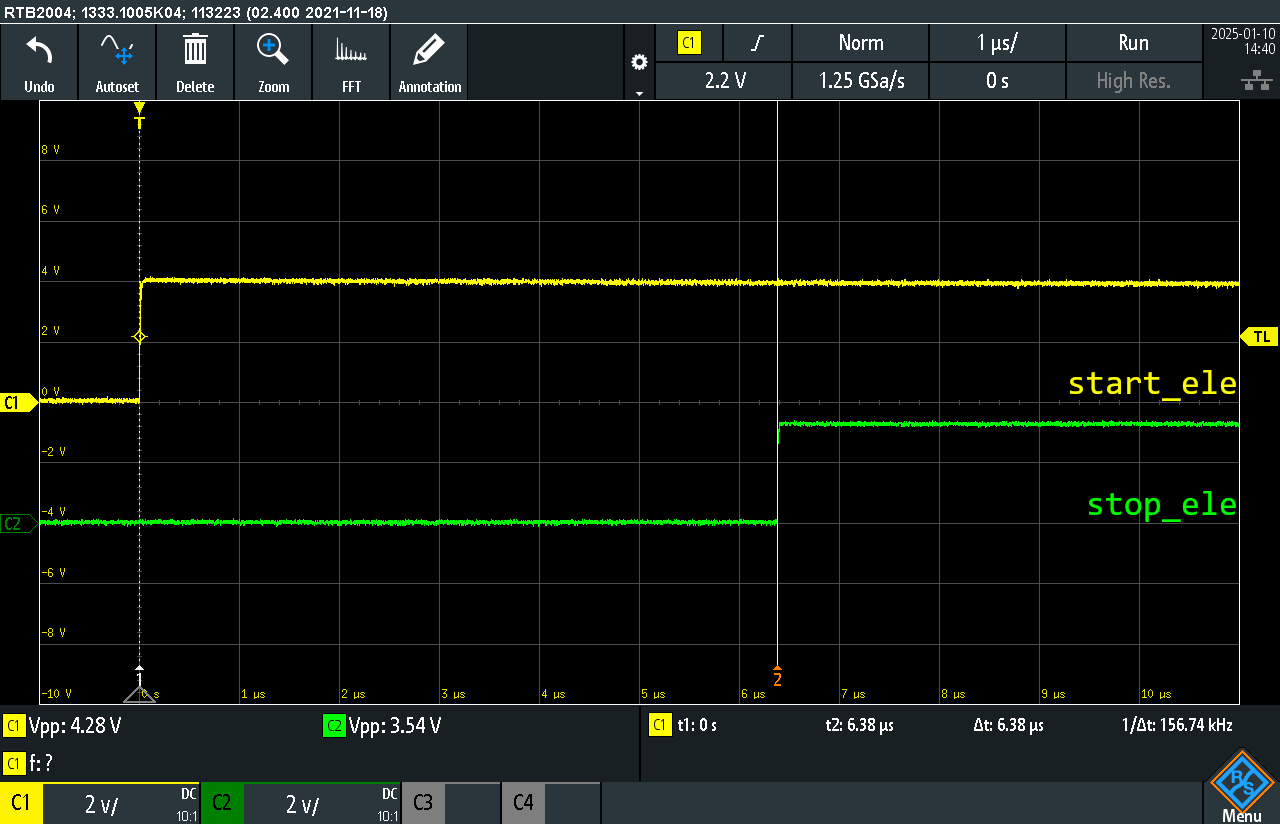
\includegraphics[width=0.8\textwidth]{graphics/gpio_toggle_with_hal_dso.png}
    \caption{\acrshort{gpio} Toggle mit \acrshort{hal} - \acrshort{dso}}\label{fig:gpio_toggle_with_hal_dso}
\end{figure}

\begin{figure}[H]
    \centering
    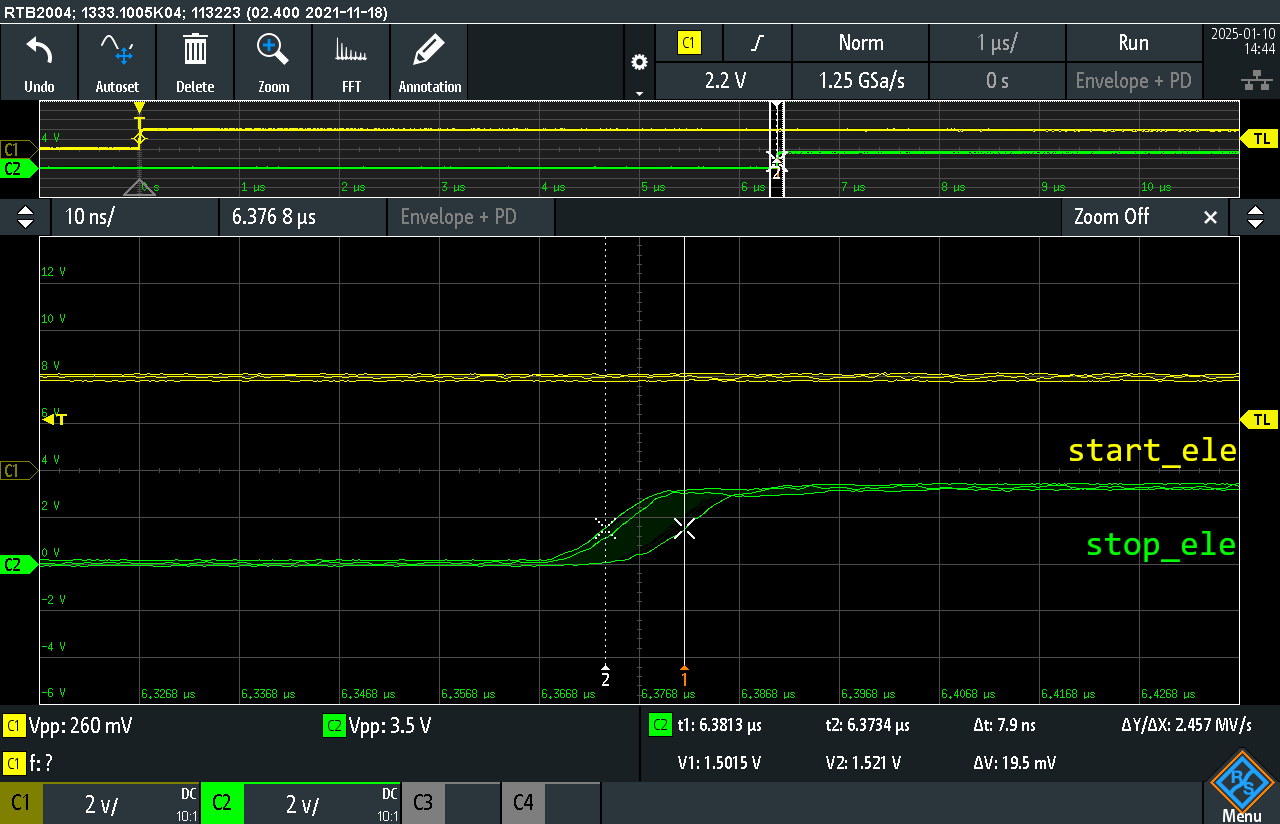
\includegraphics[width=0.8\textwidth]{graphics/gpio_toggle_with_hal_dso_zoom.png}
    \caption{\acrshort{gpio} Toggle mit \acrshort{hal} - \acrshort{dso} (Zoom)}\label{fig:gpio_toggle_with_hal_dso_zoom}
\end{figure}

\subsubsection{GPIO Toggle ohne HAL}\label{sec:gpio_toggle_without_hal}

Als nächstes wird gemessen wie lange es für die \acrshort{cpu} der \acrshort{mcu} dauert mit direktem Register-Zugriff
(via Pointer; ohne \acrshort{hal}-Library) zwei \acrshort{gpio}-Pins zu schalten.

In Code~\ref{code:gpio_toggle_without_hal} ist die Firmware-Implementation dazu gezeigt.

\lstinputlisting[language={C}, label={code:gpio_toggle_without_hal}, caption={\acrshort{gpio} Toggle ohne \acrshort{hal}}]{sourcecode/gpio_toggle_without_hal.c}

Der \acrshort{tdc} misst also die Zeit zwischen Zeile 15 und 16 in Code~\ref{code:gpio_toggle_without_hal}. Dazu wird,
wie in Kapitel \ref{sec:gpio_toggle_with_hal}, der STOP-Pin des \acrshort{tdc} via \lstinline|SW1| mit
\lstinline|stop_ele| verbunden. Der Kabelanschluss \lstinline|J3| wird kurzgeschlossen. Siehe
Abbildung~\ref{fig:tdc_ele_signal}.

Via \acrshort{uart} wurden 2000 Messwerte erfasst. Ein Ausschnitt davon ist in Code
\ref{code:gpio_toggle_without_hal_log} gezeigt. Die restlichen Daten befinden sich im elektronischen Anhang.

\lstinputlisting[language={}, label={code:gpio_toggle_without_hal_log}, caption={\acrshort{gpio} Toggle ohne \acrshort{hal}}]{sourcecode/gpio_toggle_without_hal_log.txt}

Arithmetischer Mittelwert und Standardabweichung sind in Formel \ref{eq:gpio_toggle_without_hal} aufgeführt.

\begin{equation}\label{eq:gpio_toggle_without_hal}
    \begin{split}
        \overline{ToF} &= 1'377'773~ps\\
        \sigma         &= 402~ps
    \end{split}
\end{equation}
\myequations{\acrshort{gpio} Toggle ohne \acrshort{hal}}

Da die \acrshort{cpu} mit 8~MHz läuft, lässt sich daraus schliessen, dass ein Pin-Toggle ohne \acrshort{hal} ca. 10
\acrshort{cpu}-Cycles benötigt. Dies erscheint plausibel.

Histogramm und Boxplot sind in Abbildung~\ref{fig:gpio_toggle_without_hal_histogram} bzw.
\ref{fig:gpio_toggle_without_hal_boxplot} dargestellt.

\begin{figure}[H]
    \centering
    \includesvg[width=0.8\textwidth]{graphics/gpio_toggle_without_hal_histogram.svg}
    \caption{\acrshort{gpio} Toggle ohne \acrshort{hal} - Histogramm}\label{fig:gpio_toggle_without_hal_histogram}
\end{figure}

\begin{figure}[H]
    \centering
    \includesvg[width=0.8\textwidth]{graphics/gpio_toggle_without_hal_boxplot.svg}
    \caption{\acrshort{gpio} Toggle ohne \acrshort{hal} - Boxplot}\label{fig:gpio_toggle_without_hal_boxplot}
\end{figure}

Um die Resultate des \acrshort{tdc} zu validieren, wurde dieselbe Messung auch mittels \acrfull{dso} durchgeführt. Die
Messungen sind in Abbildung~\ref{fig:gpio_toggle_without_hal_dso} und \ref{fig:gpio_toggle_without_hal_dso_zoom}
dargestellt.

\begin{figure}[H]
    \centering
    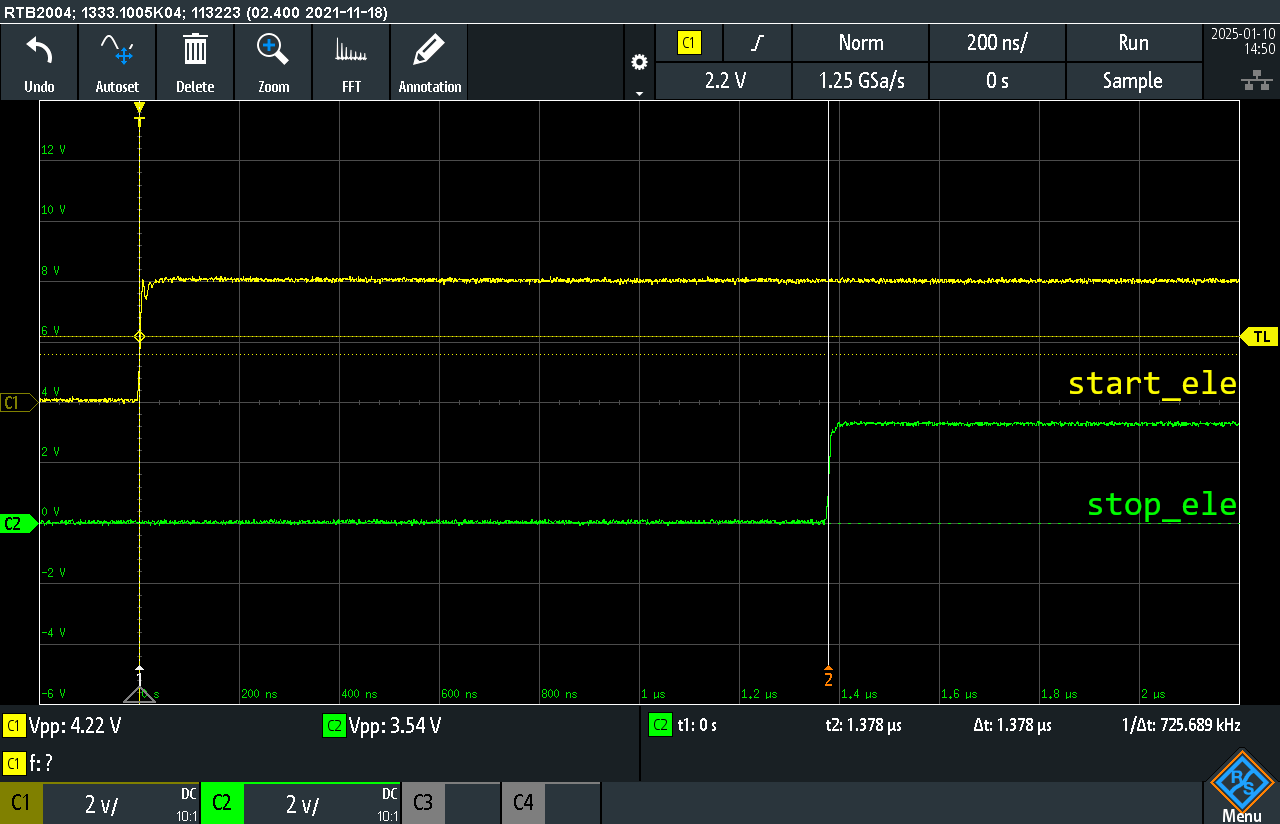
\includegraphics[width=0.8\textwidth]{graphics/gpio_toggle_without_hal_dso.png}
    \caption{\acrshort{gpio} Toggle ohne \acrshort{hal} - \acrshort{dso}}\label{fig:gpio_toggle_without_hal_dso}
\end{figure}

\begin{figure}[H]
    \centering
    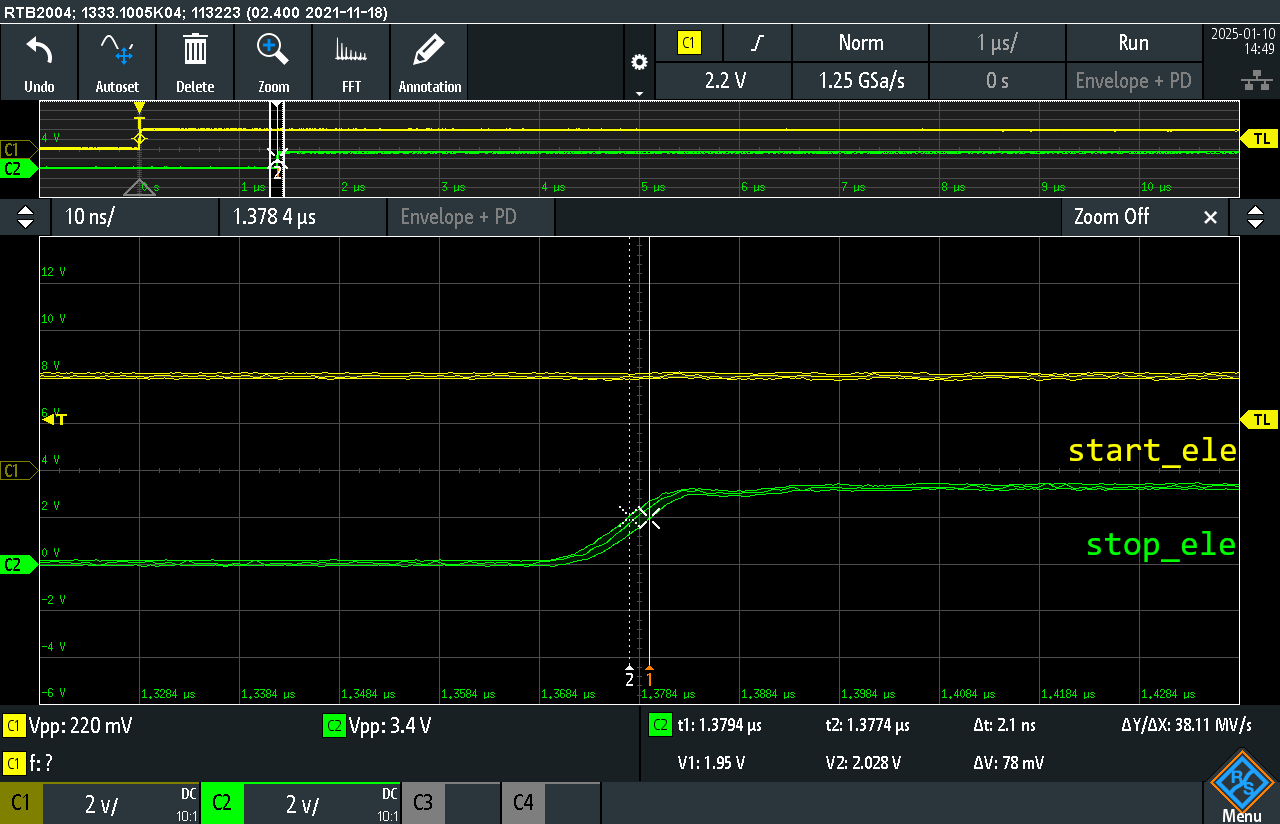
\includegraphics[width=0.8\textwidth]{graphics/gpio_toggle_without_hal_dso_zoom.png}
    \caption{\acrshort{gpio} Toggle ohne \acrshort{hal} - \acrshort{dso} (Zoom)}\label{fig:gpio_toggle_without_hal_dso_zoom}
\end{figure}

\subsubsection{Unterschiedliche Kabellängen}\label{sec:different_cable_lengths}

Für diese Messung wird dasselbe Setup wie in Kapitel \ref{sec:gpio_toggle_without_hal} verwendet.

Anstelle eines Kurzschlusses von \lstinline|J3| (siehe Abbildung \ref{fig:tdc_ele_signal}) werden nun verschiedene
Kabellängen angeschlossen.

Als Kabel wird ein einzelner, isolierter Kupferdraht ($\diameter_{cu} = 0.8~mm$, $\diameter_{ges} = 1.6~mm$) verwendet.

Es hat sich herausgestellt, dass eine kreisförmige Anordnung des Kabels wichtig ist. Denn bei einer Überlappung der
beiden Kabelenden werden kürze Zeiten gemessen. Dies hat mit der kapazitiven Kopplung zwischen den Leitern zu tun.

Die Resultate sind in Abbildung~\ref{fig:different_cable_lengths} dargestellt. Die Liste mit den Datenpunkten befindet
sich im elektronischen Anhang.

\begin{figure}[H]
    \centering
    \includesvg[width=0.9\textwidth]{graphics/different_cable_lengths.svg}
    \caption{Unterschiedliche Kabellängen}\label{fig:different_cable_lengths}
\end{figure}

Die arithmetischen Mittelwerte und Standardabweichungen sind in Tabelle \ref{tab:different_cable_lengths} aufgeführt.

\begin{table}[H]
    \mytable
        {|l|l|l|}
        {\textbf{Länge} & \textbf{Mittelwert} & \textbf{Standardabweichung}}
        {\length & \mean & \stddev}
        {tables/different_cable_lengths.csv}
    \caption{Unterschiedliche Kabellängen}\label{tab:different_cable_lengths}
\end{table}

Die Signal-Ausbreitungs-Geschwindigkeit in Kupfer beträgt ca. $\sfrac{2}{3}$ der Lichtgeschwindigkeit
\cite{firewallcx2025propagationdelay}. Um die Resultate in Tabelle \ref{tab:different_cable_lengths} zu validieren,
rechnen wir, wie in Formel \ref{eq:cable_length} gezeigt, auf die Kabellänge zurück. Die Laufzeit bei 0~m wird dabei
abgezogen, um die Verzögerung zu kompensieren, welche durch das Schalten der \acrshort{gpio}s entsteht.

\begin{equation}\label{eq:cable_length}
    \begin{split}
        c_{cu} &\approx \frac{2}{3} \cdot c_0 = \frac{2}{3} \cdot 299'792'458~\frac{m}{s} \approx 200'000'000~\frac{m}{s}\\
        ToF_{n} &= ToF_{n_{abs}} - ToF_{0}\\
        l_{n}   &= ToF_{n} \cdot c_{cu}
    \end{split}
\end{equation}
\myequations{Zurückrechnen auf Kabellänge}

Die Resultate sind in Tabelle \ref{tab:different_cable_lengths_calc} dargestellt.

\begin{table}[H]
    \mytable
        {|l|l|l|}
        {\textbf{Tatsächliche Länge} & \textbf{ToF}$\mathbf{_n}$ & \textbf{Zurückgerechnete Länge}}
        {\reallength & \tofn & \calclength}
        {tables/different_cable_lengths_calc.csv}
    \caption{Kabellängen zurückgerechnet}\label{tab:different_cable_lengths_calc}
\end{table}

Es fällt auf, dass die Resultate nicht genau übereinstimmen. Es ist jedoch eine klare Korrelation zu erkennen.

Der Unterschied könnte verschiedene Ursachen haben. Eine mögliche Erklärung wäre, dass die Ausbreitungs-Geschwindigkeit
beim verwendeten Kabel näher an der Lichtgeschwindigkeit ist als angenommen. Weitere Messresultate und Auswertungen
dazu in Kapitel~\ref{sec:different_cable_lengths_with_dso}.

\subsubsection{Mode 1 vs. Mode 2}

Der TDC7200 unterstützt zwei Modi mit unterschiedlichen Messbereichen \cite{ti2016tdc7200_datasheet}:

\begin{itemize}
    \item Mode 1: 12~ns bis 500~ns
    \item Mode 2: 250~ns bis 8~ms
\end{itemize}

Im Mode~1 wird nur der interne Ring-Oszillator des \acrshort{tdc} verwendet. Siehe dazu Abbildung~\ref{fig:tdc_mode1}.

\begin{figure}[H]
    \centering
    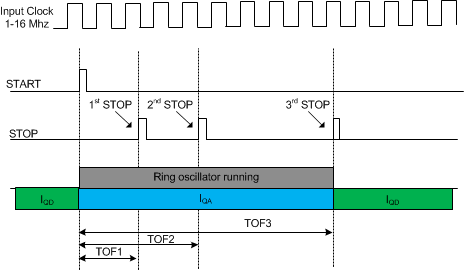
\includegraphics[width=0.6\textwidth]{graphics/tdc_mode1.png}
    \caption[\acrshort{tdc} Mode 1]{\acrshort{tdc} Mode 1 \cite{ti2016tdc7200_datasheet}}\label{fig:tdc_mode1}
\end{figure}

Im Mode~2, um längere Zeiten messen zu können, wir zusätzlich der externe Clock des \acrshort{tdc} verwendet. Siehe dazu
Abbildung~\ref{fig:tdc_mode2}.

\begin{figure}[H]
    \centering
    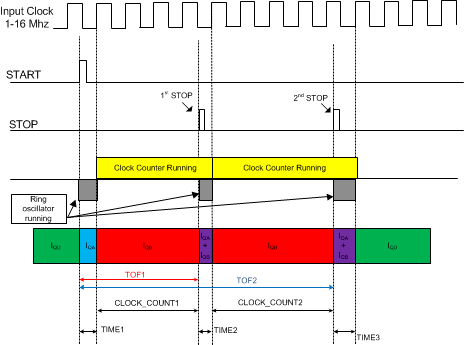
\includegraphics[width=0.6\textwidth]{graphics/tdc_mode2.png}
    \caption[\acrshort{tdc} Mode 2]{\acrshort{tdc} Mode 2 \cite{ti2016tdc7200_datasheet}}\label{fig:tdc_mode2}
\end{figure}

Die bisherigen Messungen (Kapitel~\ref{sec:gpio_toggle_with_hal}, \ref{sec:gpio_toggle_without_hal} und
\ref{sec:different_cable_lengths}) wurden im Mode~2 durchgeführt, da das Schalten der \acrshort{gpio}s mit der
\acrshort{cpu} mehr als 500~ns brauchte.

In künftigen Messungen soll das Schalten der \acrshort{gpio}s von einem Hardware-Timer der \acrshort{mcu} erledigt
werden. Damit werden Schaltzeiten von 125~ns bei 8~MHz bzw. 20.8~ns bei 48~MHz möglich sein. Es soll deshalb in diesem
Kapitel ein Vergleich der Messresultate der beiden Modi gemacht werden.

Dazu wurden drei Messungen gemacht:
\begin{enumerate}
    \item \acrshort{gpio} Toggle ohne \acrshort{hal} im Mode~2 mit Kabellänge~=~0~m (wie in Kapitel~\ref{sec:gpio_toggle_without_hal} und \ref{sec:different_cable_lengths})
    \item \acrshort{gpio} Toggle ohne \acrshort{hal} im Mode~2 mit Kabellänge~=~6~m (wie in Kapitel~\ref{sec:different_cable_lengths})
    \item Ohne GPIO Toggle Im Mode~1 mit Kabellänge~=~6~m
\end{enumerate}

Für die Messung im Mode~1 soll auf die Verzögerung durch das Schalten der \acrshort{gpio}s verzichtet werden. Dazu wird
das \lstinline|START|- und \lstinline|STOP|-Signal vom selben \acrshort{gpio}-Pin, \lstinline|start_ele|, generiert.
Dazu wird \lstinline|SW1| mit \lstinline|start_ele| verbunden (siehe Abbildung~\ref{fig:tdc_ele_signal}).

In Code~\ref{code:mode1} ist die Firmware-Implementation für eine Messung im Mode~1 gezeigt.

\lstinputlisting[language={C}, label={code:mode1}, caption={Mode 1}]{sourcecode/mode1.c}

Die Unterschiede im Vergleich zu den Messungen in Kapitel~\ref{sec:gpio_toggle_without_hal} und
\ref{sec:different_cable_lengths} sind:

\begin{itemize}
    \item Zeile 7: \acrshort{tdc} wird im Mode~1 konfiguriert (anstatt Mode~2)
    \item Zeile 15 und 23: Es wird nur der \lstinline|start_ele| Pin getoggelt (anstatt \lstinline|start_ele| und \lstinline|stop_ele| Pin)
\end{itemize}

Die Erwartung ist, dass die Differenz aus Messung~1 und Messungen~2 ungefähr dem Resultat aus Messung~3 entspricht.

Die Resultate dieser drei Messungen sind in Tabelle \ref{tab:mode1_vs_mode2} aufgeführt. Die restlichen Daten befinden
sich im elektronischen Anhang.

\begin{table}[H]
    \mytable
        {|l|l|l|}
        {\textbf{Messung} & \textbf{Mittelwert} & \textbf{Standardabweichung}}
        {\measurement & \mean & \stddev}
        {tables/mode1_vs_mode2.csv}
    \caption{Mode 1 vs. Mode 2}\label{tab:mode1_vs_mode2}
\end{table}

Die Berechnung in Formel~\ref{eq:mode1_vs_mode2} zeigt, dass die Messresultate nahe beieinander liegen.

\begin{equation}\label{eq:mode1_vs_mode2}
    \begin{split}
        \Delta Mode~2 &= 1'403'224~ps - 1'378'222~ps = 25'001~ps\\
        Mode~1        &= 25'145~ps
    \end{split}
\end{equation}
\myequations{Mode 1 vs. Mode 2}

Es kann also davon ausgegangen werden, dass Mode~1 und Mode~2 im Firmware-Treiber korrekt implementiert wurden.

Bemerkung: Im Firmware-Treiber (siehe Anhang~\ref{sec:tdc_driver}) kann für beide Modi dieselbe Funktion
\lstinline|TDC_read_result()| verwendet werden. Für Mode~1 vereinfacht sich die Berechnung, weil \lstinline|TIME2|~=~0
und \lstinline|CLOCK_COUNT1|~=~0.

\subsubsection{Timer Output}\label{sec:timer_output}

In Kapitel~\ref{sec:gpio_toggle_with_hal} und \ref{sec:gpio_toggle_without_hal} wurde gezeigt, dass es einige
\acrshort{cpu}-Cycles dauert, um  mittels Software, also mit \acrshort{cpu}-Instruktionen, \acrshort{gpio}s zu toggeln.

Eine schnellere Methode ist es, das Toggeln der \acrshort{gpio}s von der Hardware-Peripherie der \acrshort{mcu}
erledigen zu lassen. Dazu eignen sich Hardware-Timer.

In Abbildung \ref{fig:clock_config_default} ist die default Clock-Configuration des Nucleo-Boards gezeigt.

\begin{figure}[H]
    \centering
    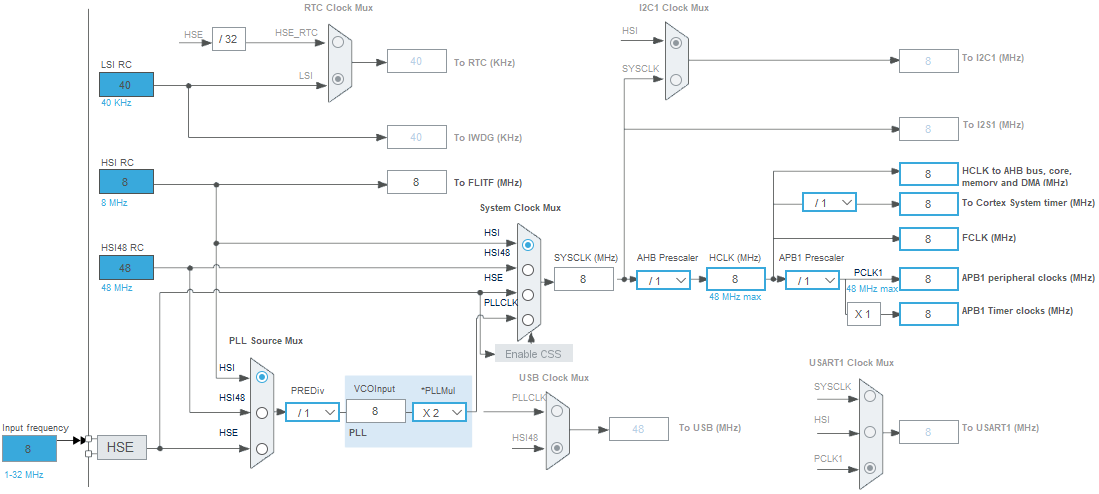
\includegraphics[width=0.9\textwidth]{graphics/clock_config_default.png}
    \caption{Default Clock-Configuration}\label{fig:clock_config_default}
\end{figure}

Per default wird der \acrfull{hsi} Clock mit 8~MHz verwendet. Damit sollte es mit Hardware-Timer möglich sein, zwei
\acrshort{gpio}s zu schalten mit einer Verzögerung gemäss Formel~\ref{eq:gpio_schalten_zeit}.

\begin{equation}\label{eq:gpio_schalten_zeit}
    t = \frac{1}{8~MHz} = 125~ns
\end{equation}
\myequations{\acrshort{gpio}-Schalten Verzögerungszeit}

Dazu werden Kanal \lstinline|CH1| und \lstinline|CH4| des Hardware-Timers \lstinline|TIM1| im Output Compare Match Modus
verwendet. Die zugeordneten \acrshort{gpio}-Pins sind \lstinline|start_ele| bzw. \lstinline|stop_ele|.

Erreicht der 16~bit Timer den Wert \lstinline|32'000| wird \lstinline|start_ele| auf High geschalten. Beim Erreichen des
Werts \lstinline|32'001| wird \lstinline|stop_ele| auf High geschalten.

Der \acrshort{tdc} wird in Mode 1 konfiguriert. Der STOP-Pin des \acrshort{tdc} wird via \lstinline|SW1| mit
\lstinline|stop_ele| verbunden. Der Kabelanschluss \lstinline|J3| wird kurzgeschlossen. Siehe
Abbildung~\ref{fig:tdc_ele_signal}.

In Code~\ref{code:timer_output} ist die Firmware-Implementation dazu gezeigt.

\lstinputlisting[language={C}, label={code:timer_output}, caption={\acrshort{gpio} Toggle mit Timer-Output}]{sourcecode/timer_output.c}

Der gemessene arithmetische Mittelwert und die Standardabweichung sind in Formel~\ref{eq:timer_output} aufgeführt.  Die
Liste mit den Datenpunkten befindet sich im elektronischen Anhang.

\begin{equation}\label{eq:timer_output}
    \begin{split}
        \overline{ToF} &=128'108~ps\\
        \sigma         &= 81~ps
    \end{split}
\end{equation}
\myequations{\acrshort{gpio} Toggle mit Timer-Output}

Erwartungsgemäss dauert das Schalten der \acrshort{gpio}s ca. 125~ns. Die Standardabweichung ist aufgrund der kleineren
Anzahl an Clock-Cycles tiefer als in den bisherigen Kapiteln.

\subsubsection{Unterschiedliche Clock-Konfigurationen}

In diesem Teilkapitel werden Messungen mit demselben Setup wie in Kapitel~\ref{sec:timer_output} durchgeführt.

Es werden die arithmetischen Mittelwerte und die Standardabweichungen verschiedener Clock-Quellen des Nucleo-Boards
verglichen. Es werden drei Messungen gemacht:

\begin{enumerate}
    \item \acrshort{hsi}: 8~MHz (wie in Kapitel~\ref{sec:timer_output})
    \item \acrshort{hsi} mit \acrshort{pll}: 16~MHz
    \item \acrshort{hsi}48: 48~MHz
\end{enumerate}

Die Clock-Konfigurationen für Messung 2 und 3 sind in Abbildung~\ref{fig:clock_config_hsi_pll_16mhz} bzw.
\ref{fig:clock_config_hsi48_48mhz} dargestellt.

\begin{figure}[H]
    \centering
    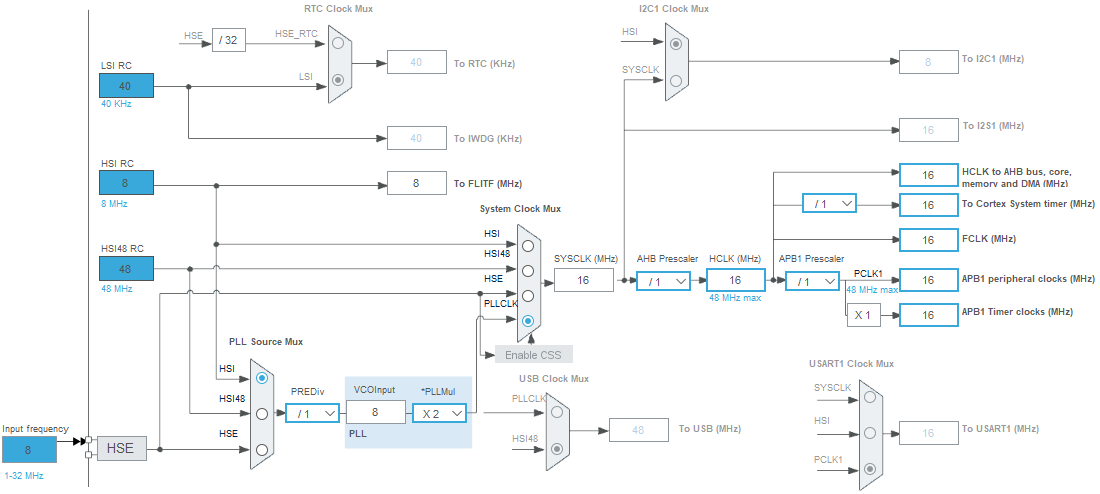
\includegraphics[width=0.9\textwidth]{graphics/clock_config_hsi_pll_16mhz.png}
    \caption{Clock-Configuration \acrshort{hsi} mit \acrshort{pll} 16~MHz}\label{fig:clock_config_hsi_pll_16mhz}
\end{figure}

\begin{figure}[H]
    \centering
    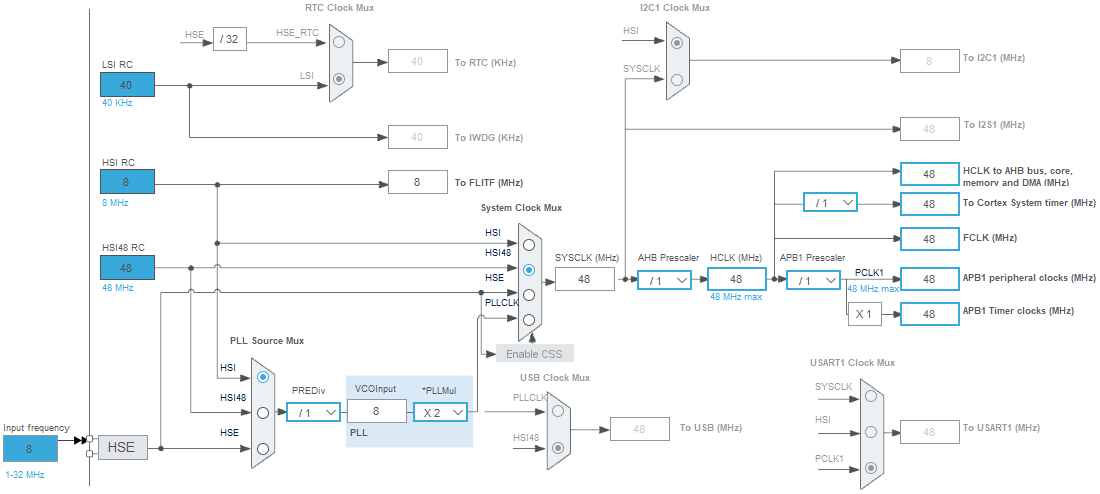
\includegraphics[width=0.9\textwidth]{graphics/clock_config_hsi48_48mhz.png}
    \caption{Clock-Configuration \acrshort{hsi}48 48~MHz}\label{fig:clock_config_hsi48_48mhz}
\end{figure}

Die arithmetischen Mittelwerte und Standardabweichungen sind in Tabelle~\ref{tab:different_clock_sources} dargestellt.
Die Liste mit den Datenpunkten befindet sich im elektronischen Anhang.

\begin{table}[H]
    \mytable
        {|l|l|l|}
        {\textbf{Messung} & \textbf{Mittelwert} & \textbf{Standardabweichung}}
        {\measurement & \mean & \stddev}
        {tables/different_clock_sources.csv}
    \caption{Unterschiedliche Clock-Quellen}\label{tab:different_clock_sources}
\end{table}

Die Resultate stimmen ungefähr mit den erwarteten Werten aus Formel~\ref{eq:gpio_schalten_zeiten} überein.

\begin{equation}\label{eq:gpio_schalten_zeiten}
    \begin{split}
        t_1 &= \frac{1}{8~MHz} = 125~ns\\
        t_2 &= \frac{1}{16~MHz} = 62.5~ns\\
        t_3 &= \frac{1}{48~MHz} = 20.8~ns
    \end{split}
\end{equation}
\myequations{\acrshort{gpio}-Schalten Verzögerungszeiten}

Im Datenblatt konnte eine Angabe zum \acrshort{pll}-Jitter gefunden werden, siehe Abbildung~\ref{fig:pll_jitter}.

\begin{figure}[H]
    \centering
    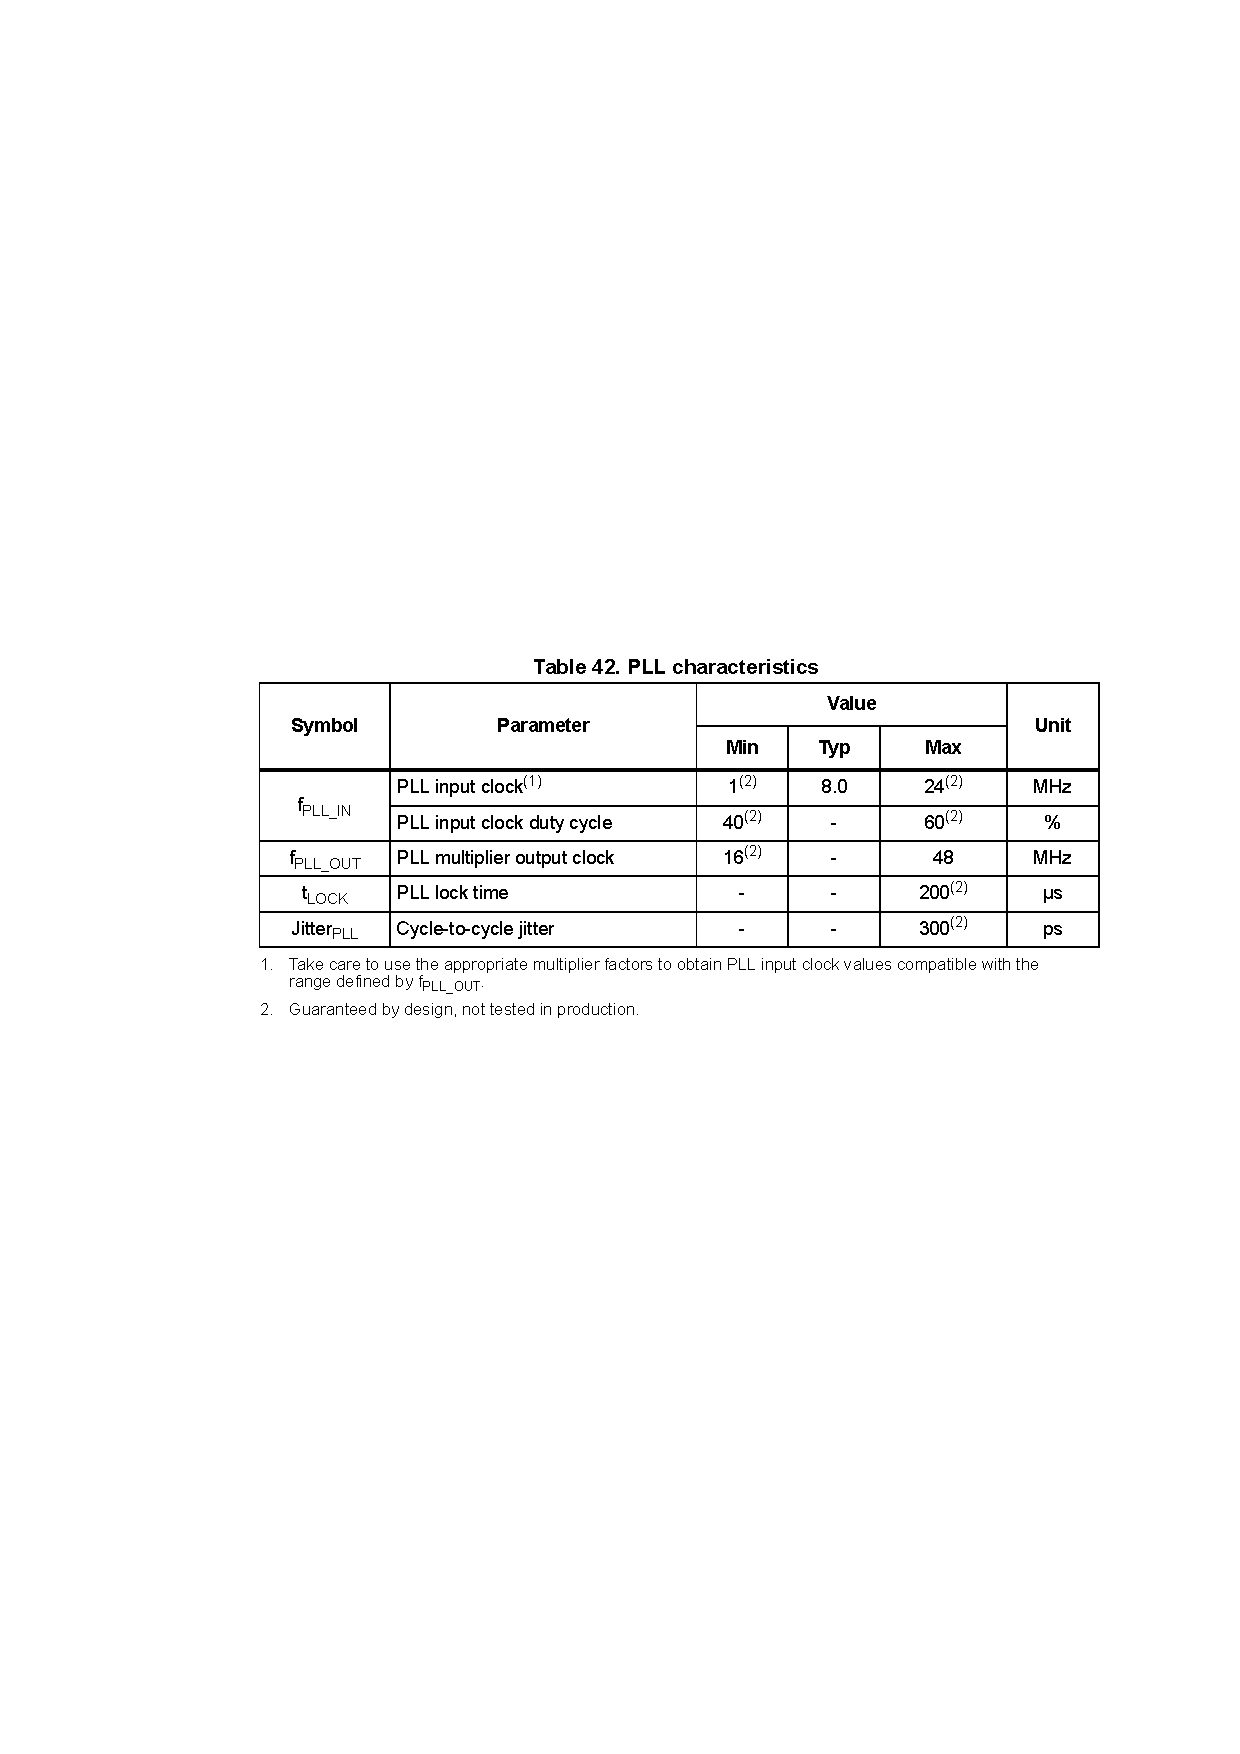
\includegraphics[width=0.8\textwidth]{graphics/pll_jitter.pdf}
    \caption[\acrshort{pll}-Jitter]{\acrshort{pll}-Jitter \cite{st2017stm32f042k6_datasheet}}\label{fig:pll_jitter}
\end{figure}

Diese Angabe ist ungefähr in derselben Grössenordnung wie die Messresultate.

\subsubsection{Unterschiedliche Kabellängen mit DSO}\label{sec:different_cable_lengths_with_dso}

In diesem Unterkapitel werden nochmals dieselben Kabellängen wie in Kapitel~\ref{sec:different_cable_lengths}
ausgemessen.

Es wird die folgende Firmware-Konfiguration verwendet, um den Jitter zu reduzieren:

\begin{itemize}
    \item \acrshort{tdc}: Modus 1
    \item Clock: 48~MHz
    \item Schalten der \acrshort{gpio}s: Timer Output
\end{itemize}

Zusätzlich werden die verschiedenen Kabellängen gleichzeitig auch via \acrshort{dso} (Rohde \& Schwarz RTB2004 2.5 GSa/s.)
ausgemessen, um die Resultate des \acrshort{tdc} damit zu vergleichen.

In Abbildung~\ref{fig:different_cable_lengths_with_dso_tdc} sind die erfassten Messresultate des \acrshort{tdc}
dargestellt. Während dem Erfassen der Messwerte war das \acrshort{dso} an den Pins angeschlossen. Die Liste mit den
Datenpunkten befindet sich im elektronischen Anhang.

\begin{figure}[H]
    \centering
    \includesvg[width=0.9\textwidth]{graphics/different_cable_lengths_with_dso_tdc.svg}
    \caption{Unterschiedliche Kabellängen - Messwerte \acrshort{tdc}}\label{fig:different_cable_lengths_with_dso_tdc}
\end{figure}

In Tabelle~\ref{tab:different_cable_lengths_with_dso_tdc} sind die Mittelwerte und die Standardabweichungen der
erfassten Messresultate des \acrshort{tdc} aufgelistet.

\begin{table}[H]
    \mytable
        {|l|l|l|l|}
        {\textbf{Länge} & \textbf{Mittelwert} & \textbf{Standardabweichung} & \textbf{$\Delta$ zu 0~m}}
        {\length & \mean & \stddev & \diff}
        {tables/different_cable_lengths_with_dso_tdc.csv}
    \caption{Unterschiedliche Kabellängen - Resultate \acrshort{tdc}}\label{tab:different_cable_lengths_with_dso_tdc}
\end{table}

In Tabelle~\ref{tab:different_cable_lengths_with_dso_dso} sind die erfassten Messresultate des \acrshort{dso}
aufgelistet. Die letzte Spalte zeigt den Unterschied zwischen \acrshort{dso} und \acrshort{tdc}. Es ist zu erkennen,
dass der Unterschied sehr klein ist.

\begin{table}[H]
    \mytable
        {|l|l|l|l|}
        {\textbf{Länge} & \textbf{Wert} & \textbf{$\Delta$ zu 0~m} & \textbf{$\Delta$ zu TDC}}
        {\length & \measurement & \diff & \difftdc}
        {tables/different_cable_lengths_with_dso_dso.csv}
    \caption{Unterschiedliche Kabellängen - Resultate \acrshort{dso}}\label{tab:different_cable_lengths_with_dso_dso}
\end{table}

Tabelle~\ref{tab:different_cable_lengths_with_dso_theorie} zeigt die theoretisch zu erwartenden Laufzeiten bei den
unterschiedlichen Annahmen für die Signalausbreitungs-Geschwindigkeiten von $\sfrac{2}{3}~c$ und $c$.

\begin{table}[H]
    \mytable
        {|l|l|l|}
        {\textbf{Länge} & \textbf{Theorie} $\mathbf{\sfrac{2}{3}~c}$ & \textbf{Theorie c}}
        {\length & \theoriekc & \theoriec}
        {tables/different_cable_lengths_with_dso_theorie.csv}
    \caption{Unterschiedliche Kabellängen - Theoretische Erwartung}\label{tab:different_cable_lengths_with_dso_theorie}
\end{table}

Die Unterschiede der \acrshort{tdc}-Resultate zu den theoretischen Erwartungen sind in den
Tabellen~\ref{tab:different_cable_lengths_with_dso_theorie_vs_tdc_ns} und
\ref{tab:different_cable_lengths_with_dso_theorie_vs_tdc_m} dargestellt. Zuerst im Bezug auf den Laufzeit-Unterschied,
dann die zurückgerechnete Kabellänge.

\begin{table}[H]
    \mytable
        {|l|l|l|}
        {\textbf{Länge} & \textbf{$\Delta$ TDC zu Theorie} $\mathbf{\sfrac{2}{3}~c}$ & \textbf{$\Delta$ TDC Theorie zu c}}
        {\length & \tdczutheoriekc & \tdczutheoriec}
        {tables/different_cable_lengths_with_dso_theorie_vs_tdc_ns.csv}
    \caption{Unterschiedliche Kabellängen - Unterschied \acrshort{tdc} [ns] zu Theorie}\label{tab:different_cable_lengths_with_dso_theorie_vs_tdc_ns}
\end{table}

\begin{table}[H]
    \mytable
        {|l|l|l|}
        {\textbf{Länge} & \textbf{TDC gem. Theorie} $\mathbf{\sfrac{2}{3}~c}$ & \textbf{TDC gem. Theorie c}}
        {\length & \tdcgemtheoriekc & \tdcgemtheoriec}
        {tables/different_cable_lengths_with_dso_theorie_vs_tdc_m.csv}
    \caption{Unterschiedliche Kabellängen - \acrshort{tdc} [m] gem. Theorie}\label{tab:different_cable_lengths_with_dso_theorie_vs_tdc_m}
\end{table}

In Tabelle~\ref{tab:different_cable_lengths_with_dso_theorie_vs_tdc_m} ist zu erkennen, dass keine der beiden
theoretischen Werte für $c$ zu einem perfekten \acrshort{tdc}-Resultat für die zurückgerechnete Distanz [m] führt.

In Tabelle~\ref{tab:different_cable_lengths_with_dso_theorie_vs_tdc_ns} ist zu erkennen, dass die Differenz der
\acrshort{tdc}-Resultate zur theoretisch zu erwartenden Laufzeit bei $c$ etwas kleiner ist als bei $\sfrac{2}{3}~c$. Es
scheint, dass $c$ eine etwas bessere Näherung darstellt.

Falls sich der gemessene Unterschied tatsächliche durch eine falsche Annahme der Ausbreitungs-Geschwindigkeit erklären
lässt, dann müsste die Ausbreitungs-Geschwindigkeit im gewählten Kabel bei ca. $0.9~c$ liegen. Die zurückrechneten
Resultate dazu sind in Tabelle~\ref{tab:different_cable_lengths_with_dso_theorie09_vs_tdc_m} aufgelistet.

\begin{table}[H]
    \mytable
        {|l|l|}
        {\textbf{Länge} & \textbf{TDC gem. Theorie 0.9 c}}
        {\length & \tdcgemtheoriemc}
        {tables/different_cable_lengths_with_dso_theorie09_vs_tdc_m.csv}
    \caption{Unterschiedliche Kabellängen - \acrshort{tdc} [m] gem. Theorie 0.9 c}\label{tab:different_cable_lengths_with_dso_theorie09_vs_tdc_m}
\end{table}

In den Abbildungen~\ref{fig:different_cable_lengths_with_dso_1m} und \ref{fig:different_cable_lengths_with_dso_6m} sind
die \acrshort{dso}-Aufzeichnungen bei den Kabellängen 1~m bzw. 6~m gezeigt. Die restlichen \acrshort{dso}-Aufzeichnungen
befinden sich im elektronischen Anhang.

\begin{figure}[H]
    \centering
    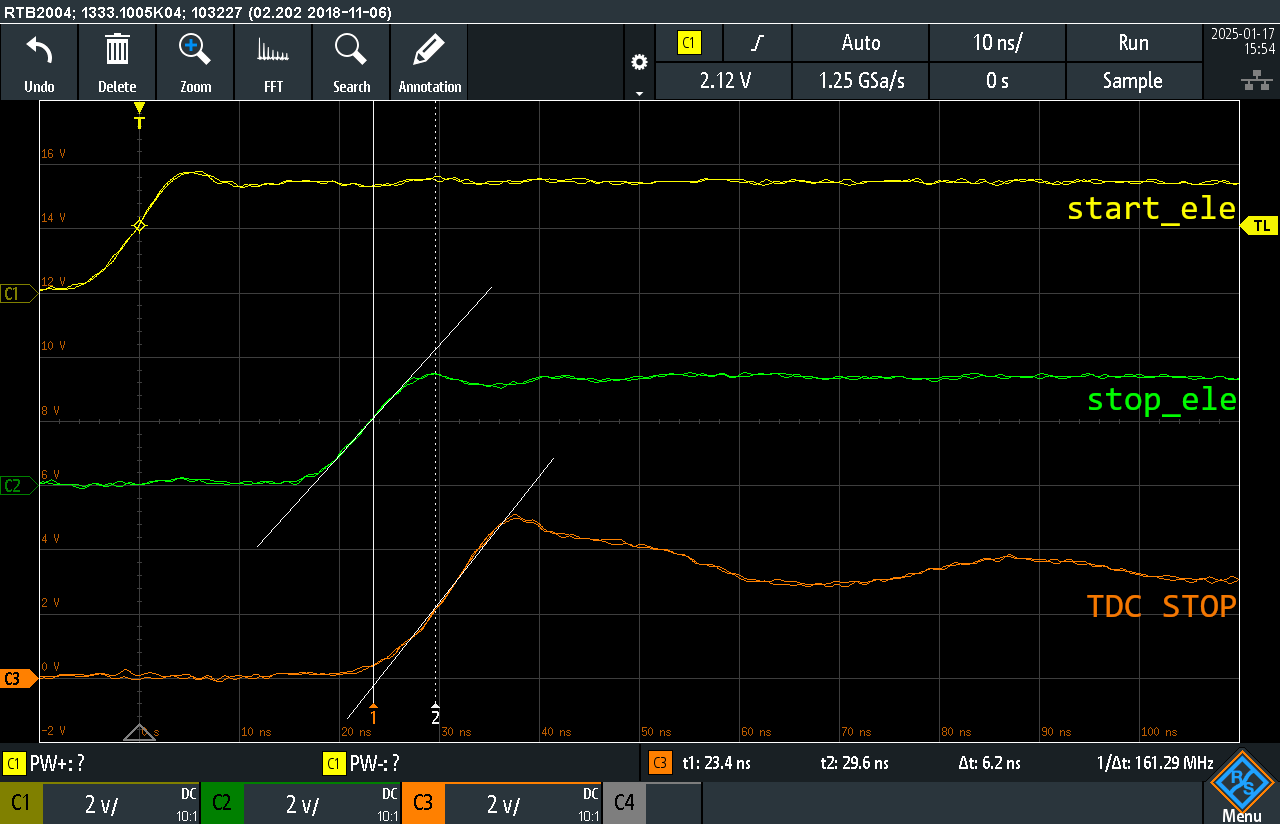
\includegraphics[width=\textwidth]{graphics/different_cable_lengths_with_dso_1m.png}
    \caption{\acrshort{dso}-Aufzeichnung bei Kabellänge 1~m}\label{fig:different_cable_lengths_with_dso_1m}
\end{figure}

\begin{figure}[H]
    \centering
    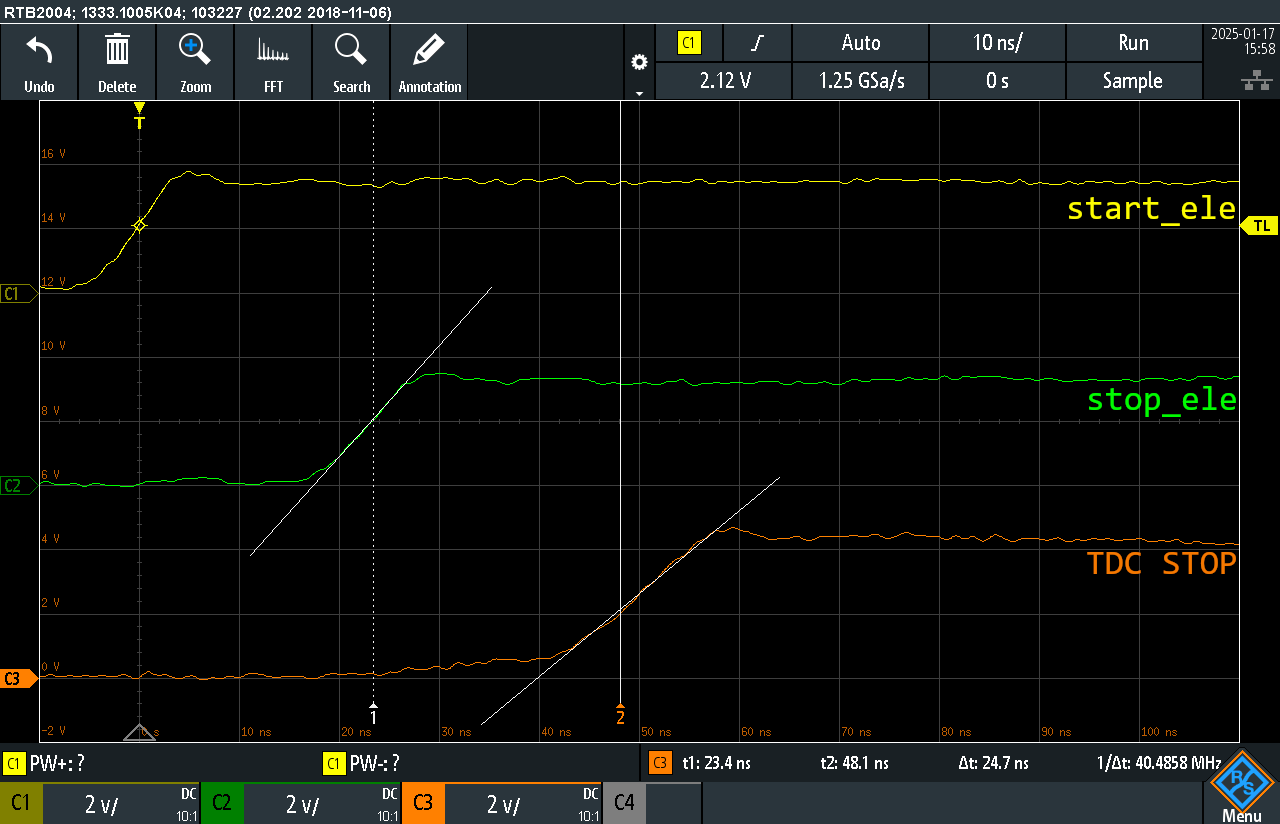
\includegraphics[width=\textwidth]{graphics/different_cable_lengths_with_dso_6m.png}
    \caption{\acrshort{dso}-Aufzeichnung bei Kabellänge 6~m}\label{fig:different_cable_lengths_with_dso_6m}
\end{figure}

Es ist zu erkennen, dass die Flanke des \lstinline|STOP|-Signals bei grösserer Kabellänge etwas abflacht. Dies hat einen
Einfluss auf die Laufzeit-Messung. Steilere Flanken würden helfen diesen Einfluss zu minimieren. Mehr dazu in
Kapitel~\ref{sec:ausblick}.

\pagebreak

\subsection{Optische Messungen}

In diesem Teilkapitel werden die Messresultate dokumentiert, welche sich auf den optischen Pfad des Demonstrators
beziehen.

Das verwendete \acrshort{dso} ist ein Rohde \& Schwarz RTB2004 2.5 GSa/s.

Für die Messungen in diesem Kapitel werden die folgenden Firmware-Konfigurationen verwendet:

\begin{itemize}
    \item \acrshort{tdc}: Modus 1
    \item Clock: 48~MHz
    \item Schalten der \acrshort{gpio}s: Timer Output
\end{itemize}

\subsubsection{Signalpfad Sender}\label{sec:messungen_signalpfad_sender}

In diesem Unterkapitel wird der Signalpfad des optischen Sendeteils ausgemessen.

Die Verzögerungszeiten zwischen den \acrshort{mcu}-Signalen \lstinline|start_op| und \lstinline|LD_pulse| sowie dem
Potential am Gate des NexFET (\lstinline|V1| Pin \lstinline|4| in Abbildung~\ref{fig:laser_driver}) sind in
Abbildung~\ref{fig:signalpfad_sender_startopt_ldpulse_fetgate} dargestellt.

\begin{figure}[H]
    \centering
    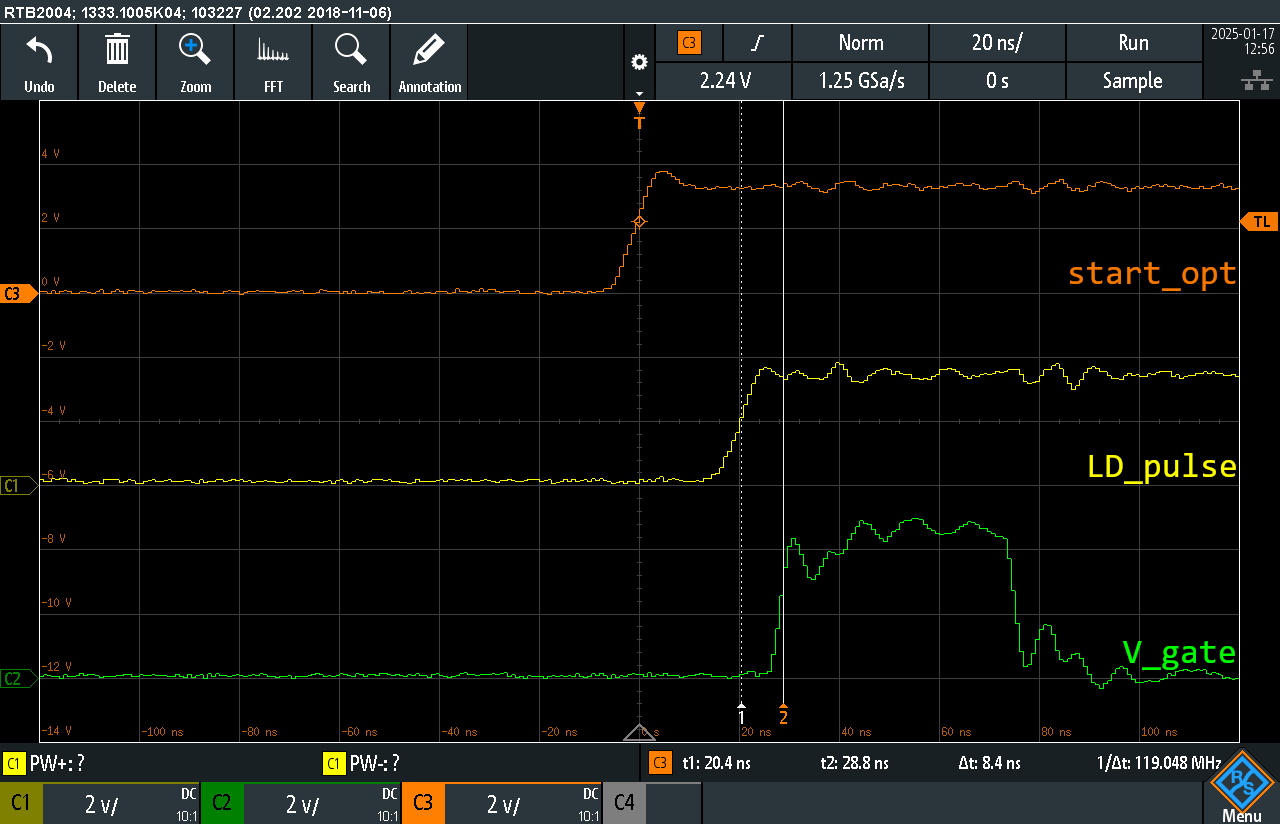
\includegraphics[width=\textwidth]{graphics/signalpfad_sender_startopt_ldpulse_fetgate.png}
    \caption{Messung Signalpfad Sender: \lstinline|start_op|, \lstinline|LD_pulse|, FET-Gate}\label{fig:signalpfad_sender_startopt_ldpulse_fetgate}
\end{figure}

Die gemessene Verzögerungszeit von 20.4~ns (20.8~ns entsprechen einem Clock-Cycle bei 48~MHz) zwischen
\lstinline|start_op| und \lstinline|LD_pulse| wurde bewusst eingefügt, um sicherzustellen, dass die minimale Messdauer
von 12~ns \cite{ti2016tdc7200_datasheet} im Mode~1 garantiert immer eingehalten wird.

Die gemessene Verzögerungszeit von 8.4~ns zwischen \lstinline|LD_pulse| und dem FET-Gate (dies entspricht dem Ausgang
des Gate-Treibers \lstinline|IC22|) ist klein und zeigt eine steile Flanke.

In Abbildung~\ref{fig:signalpfad_sender_ld_strom} ist der Strom durch die Laser-Diode (\lstinline|LD1| in
Abbildung~\ref{fig:laser_driver}) aufgezeigt.

\begin{figure}[H]
    \centering
    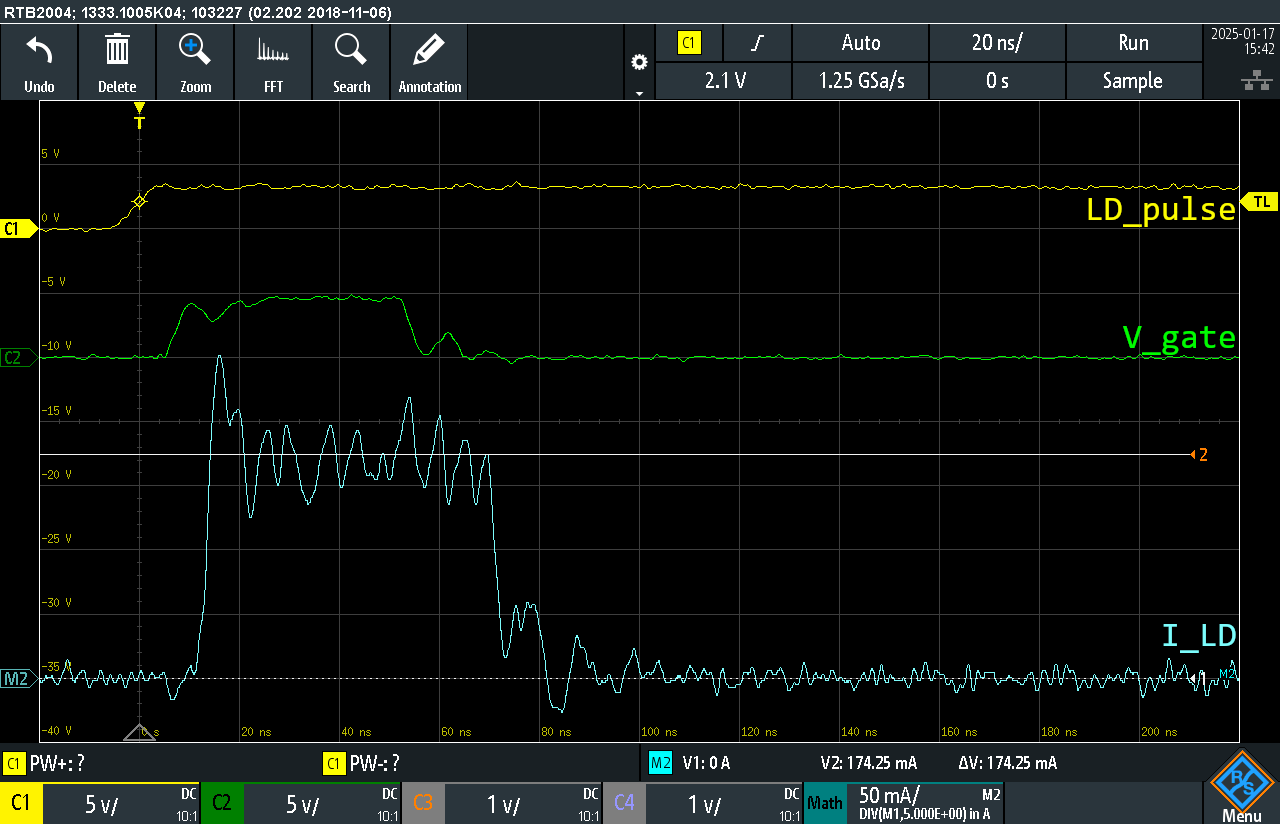
\includegraphics[width=\textwidth]{graphics/signalpfad_sender_ld_strom}
    \caption{Messung Signalpfad Sender: Strom durch Laser-Diode}\label{fig:signalpfad_sender_ld_strom}
\end{figure}

Der Strom wurde gemäss Formel~\ref{eq:messung_strom_ld} berechnet.

\begin{equation}\label{eq:messung_strom_ld}
    I_{LD} = \frac{V(\text{\lstinline|TP8|}) - V(\text{\lstinline|TP9|})}{R_V} = \frac{V(\text{\lstinline|TP8|}) - V(\text{\lstinline|TP9|})}{5~\Omega}
\end{equation}
\myequations{Berechnung Strom durch Laser-Diode}

Damit die Verzögerungszeit ersichtlich ist, wurde zusätzlich, wie in Abbildung~\ref{fig:signalpfad_sender_startopt_ldpulse_fetgate},
das Signal \lstinline|LD_pulse| und das Potential am FET-Gate aufgezeichnet.

Der gemessene Strom während dem Senden beträgt ca. 174~mA.

Dies ist um einiges weniger als der erwartete Strom von 440~mA aus Formel~\ref{eq:rld65nzx1_higher_output}. Dies hat mit
der erhöhten Dioden-Spannung zu tun. Während dem Senden erhöht sich die Spannung über der Laser-Diode auf ca. 4~V, die
Spannung über Drain-Source des FET ist vernachlässigbar klein. Damit ergibt sich der Strom durch die Diode gemäss
Formel~\ref{eq:strom_ld_tatsaechlich}.

\begin{equation}\label{eq:strom_ld_tatsaechlich}
    I_{LD} = \frac{5~V - V_{LD} - V_{DS}}{R_V} \approx \frac{5~V - 4~V}{5~\Omega} \approx 200~mA
\end{equation}
\myequations{Berechnung Strom durch Laser-Diode (tatsächlich)}

\subsubsection{ToF-Messungen via Spiegel}\label{sec:messungen_spiegel}

Damit die Photo-Diode ein möglichst starkes Signal erhält, wurde anstelle einer Wand für diese Messungen ein Spiegel
verwendet. Das Setup ist in Abbildung~\ref{fig:spiegel_setup} dargestellt.

\begin{figure}[H]
    \centering
    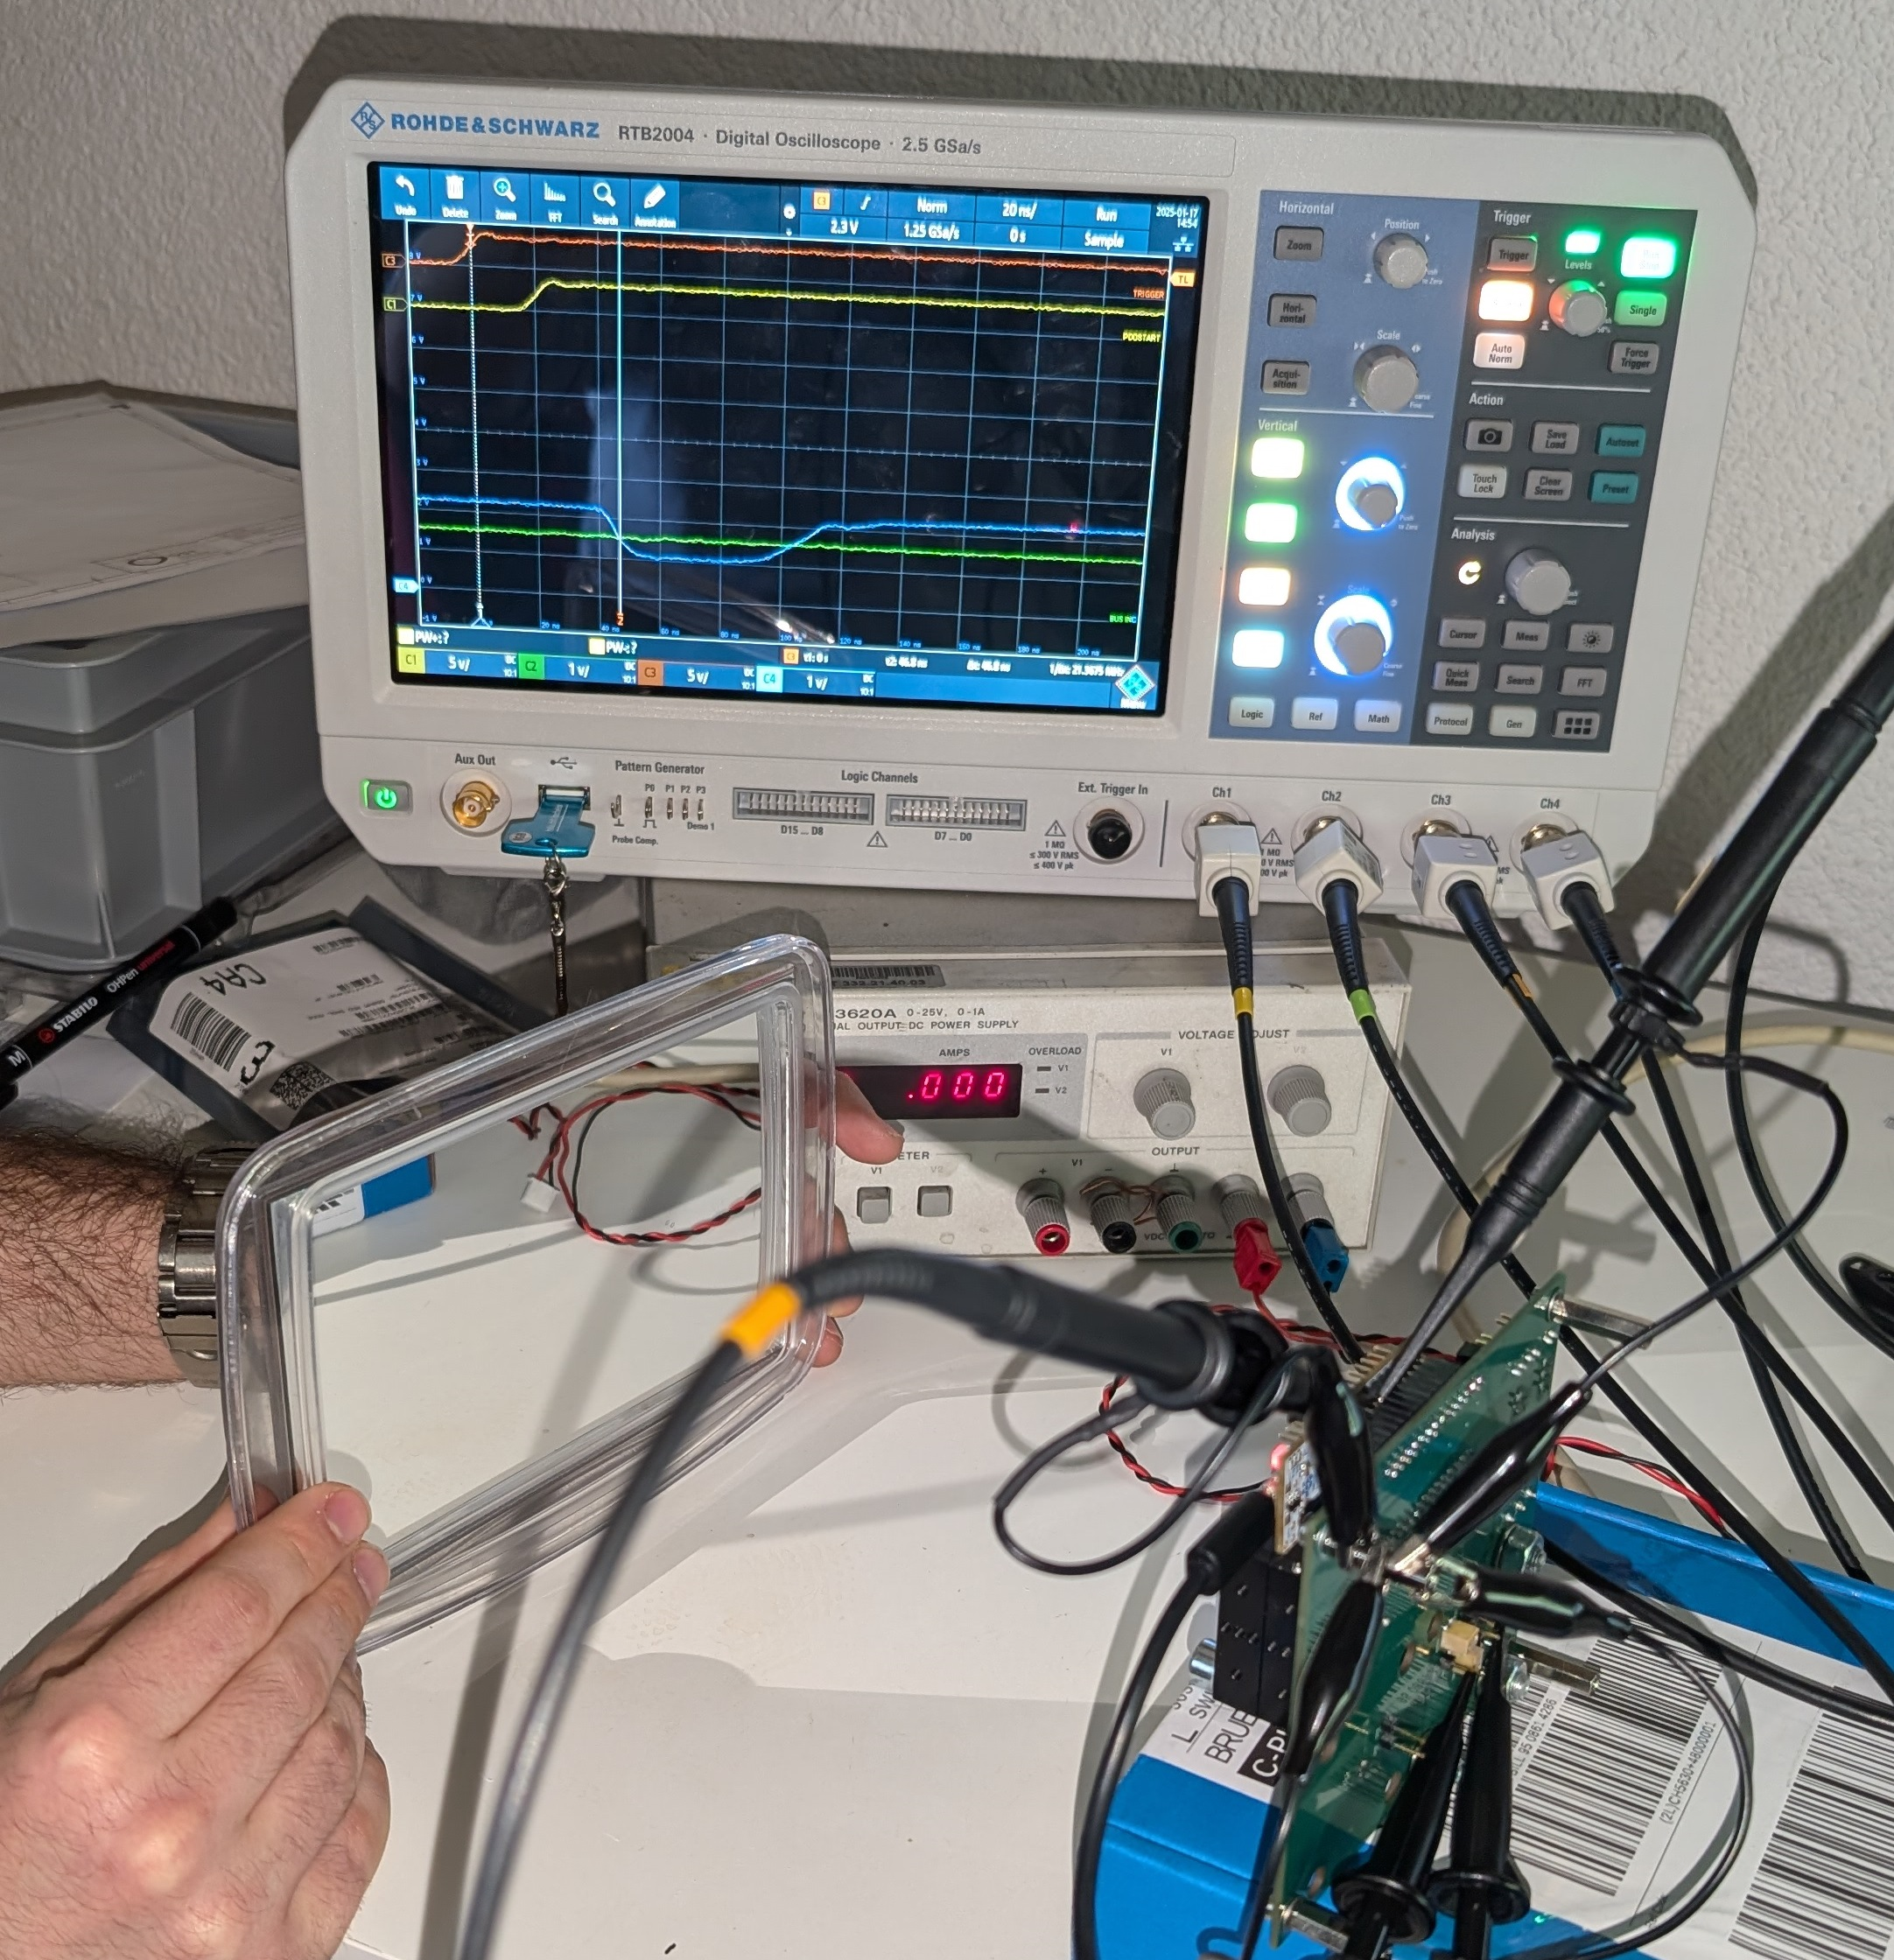
\includegraphics[width=0.6\textwidth]{graphics/spiegel_setup.jpg}
    \caption{Mess-Setup mit Spiegel}\label{fig:spiegel_setup}
\end{figure}

Gemäss Datenblatt hat die Laser-Diode eine nicht ideal punktförmige Abstrahl-Charakteristik, siehe
Abbildung~\ref{fig:laser_abstrahl_charakteristik}.

\begin{figure}[H]
    \centering
    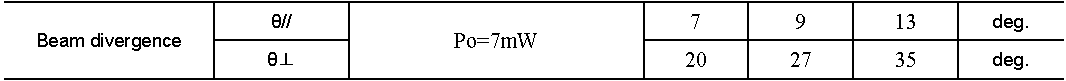
\includegraphics[width=0.8\textwidth]{graphics/laser_abstrahl_charakteristik.pdf}
    \caption[Laser Abstrahl-Charakteristik]{Laser Abstrahl-Charakteristik \cite{rohm2019rld65nzx1_datasheet}}\label{fig:laser_abstrahl_charakteristik}
\end{figure}

Es ist aufgefallen, dass mit dem gewählten \acrshort{pcb}-Layout die Orientierung der Laser-Diode für eine Spiegel-
Messung nicht ganz ideal ist. Der breitere Abstrahlwinkel ist senkrecht zur Linie zwischen Laser- und Photodiode. Siehe
dazu Abbildung~\ref{fig:laser_ausrichtung}.

\begin{figure}[H]
    \centering
    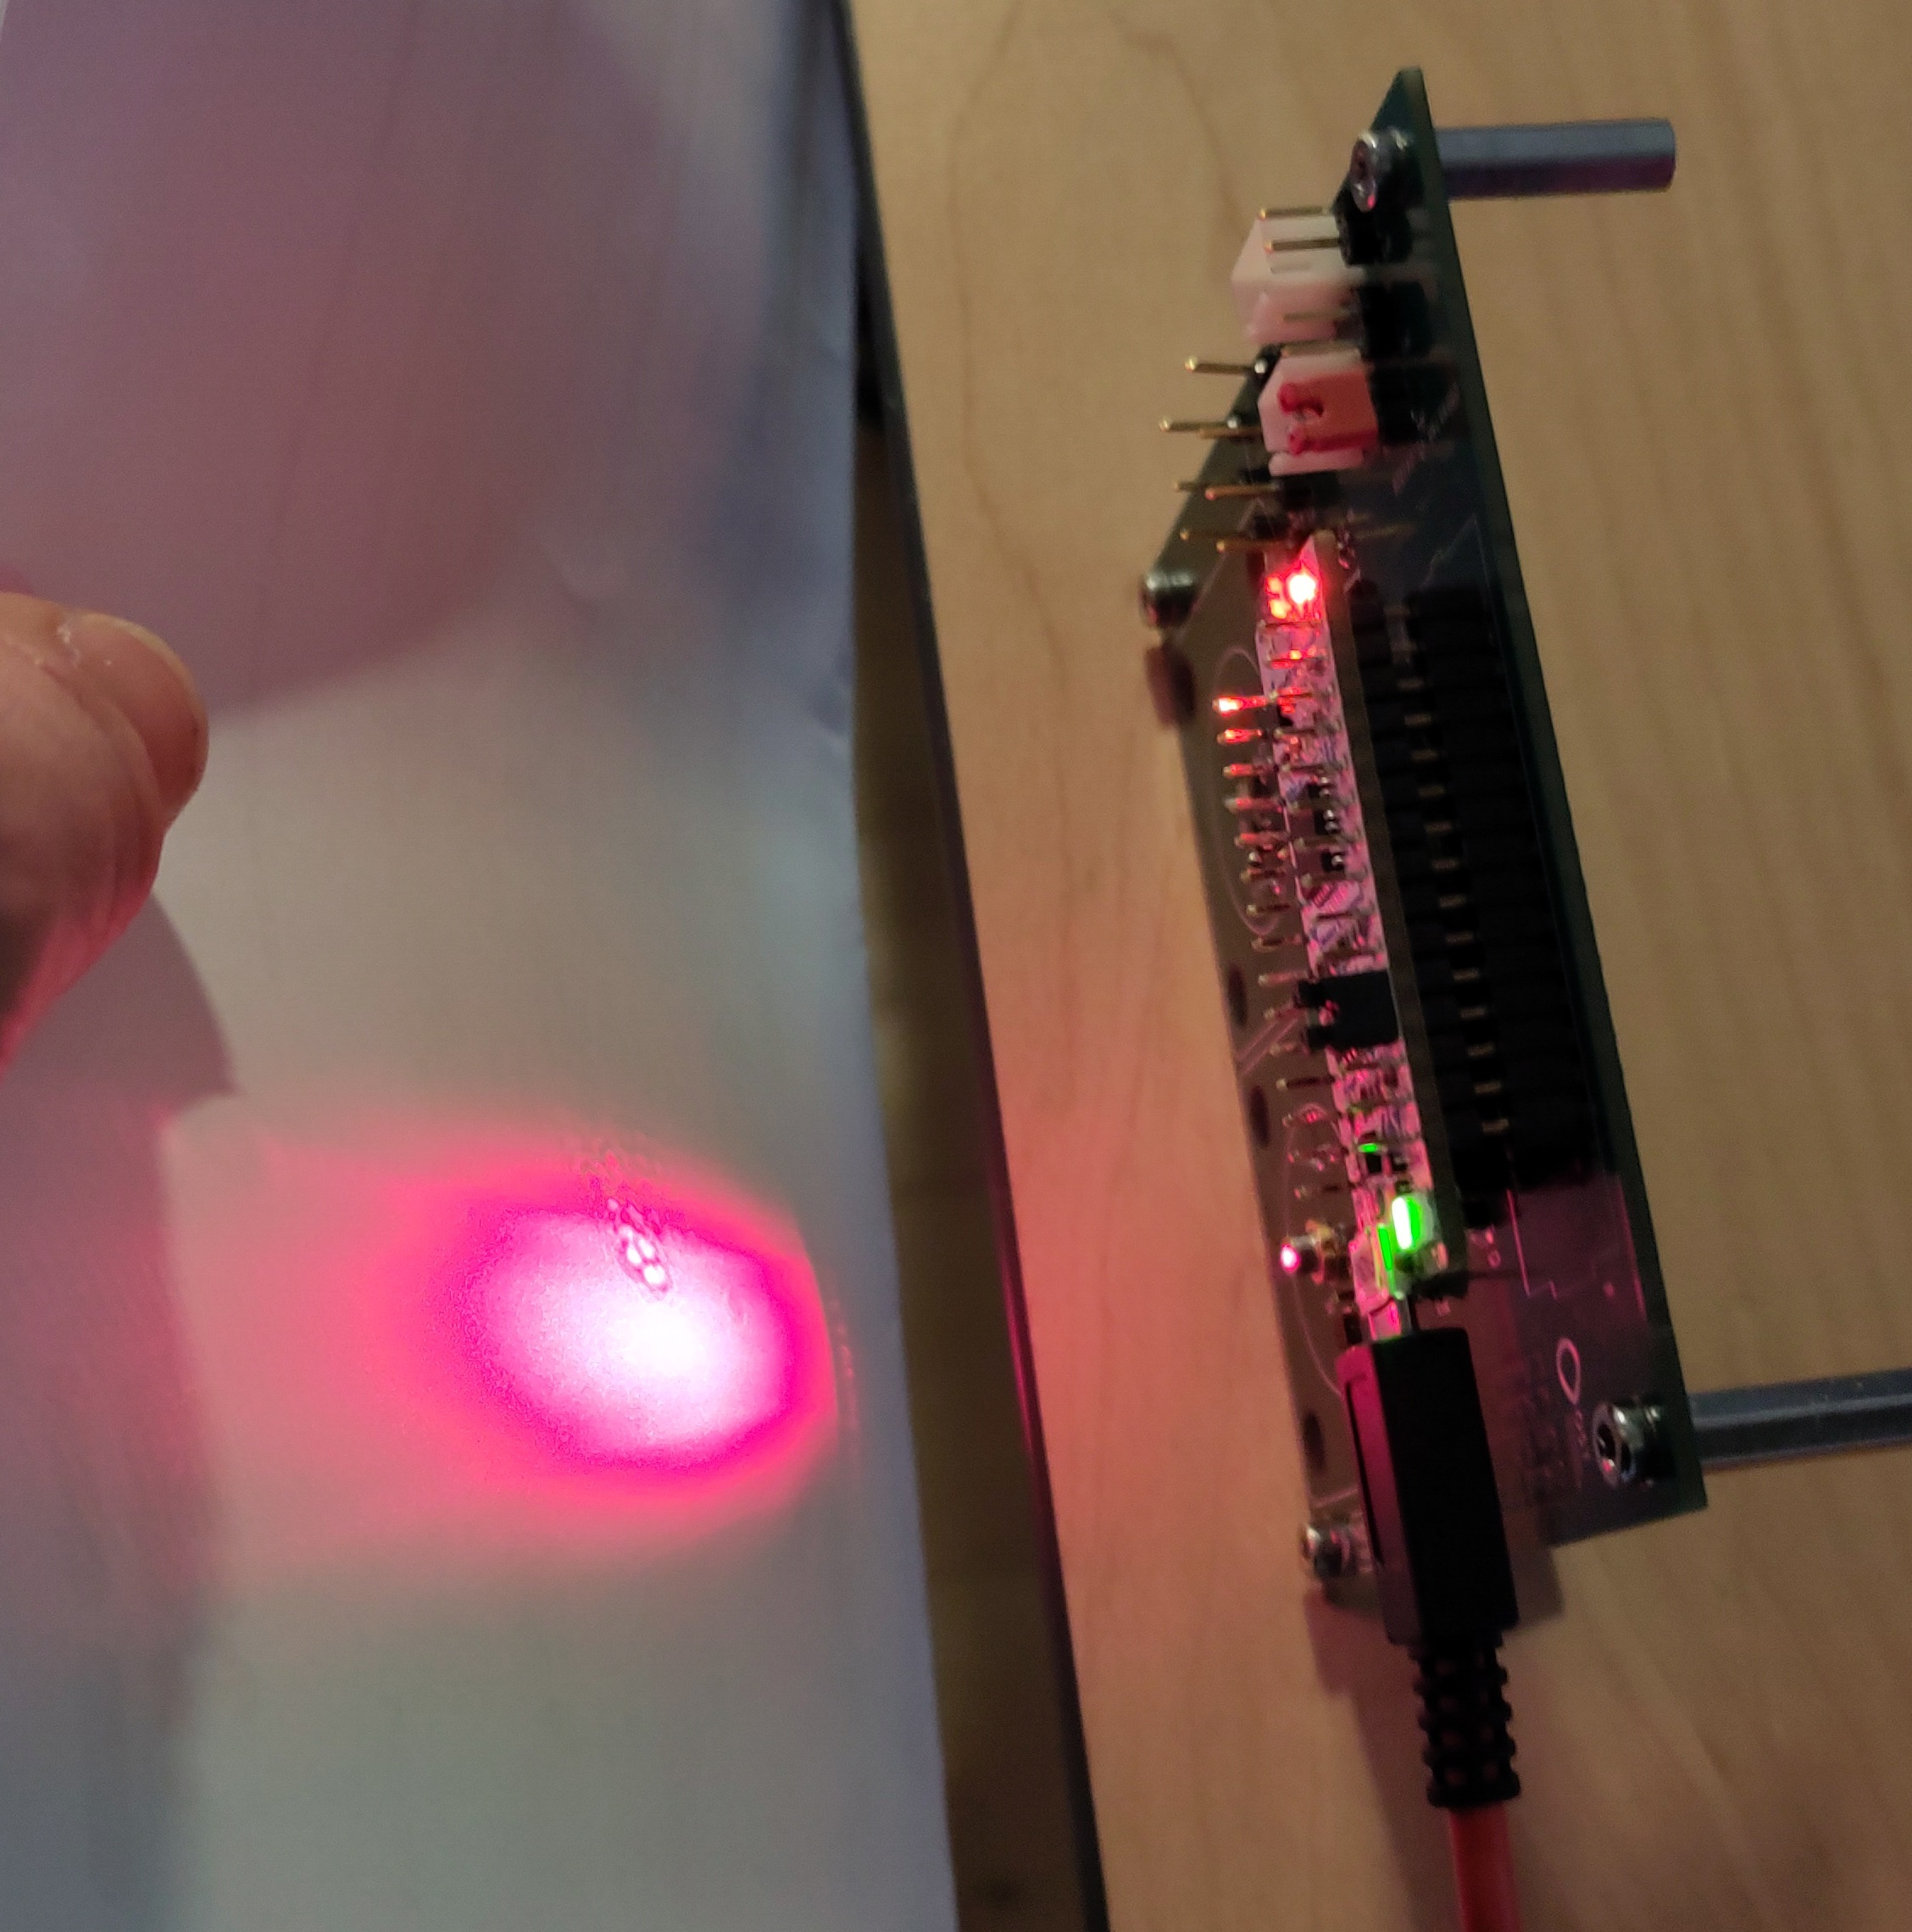
\includegraphics[width=0.6\textwidth]{graphics/laser_ausrichtung.jpg}
    \caption{Laser-Ausrichtung}\label{fig:laser_ausrichtung}
\end{figure}

Die Laser-Diode wurde deshalb manuell um $90\degree$ gedreht, wie in Abbildung~\ref{fig:laser_ausrichtung_angepasst}
dargestellt.

\begin{figure}[H]
    \centering
    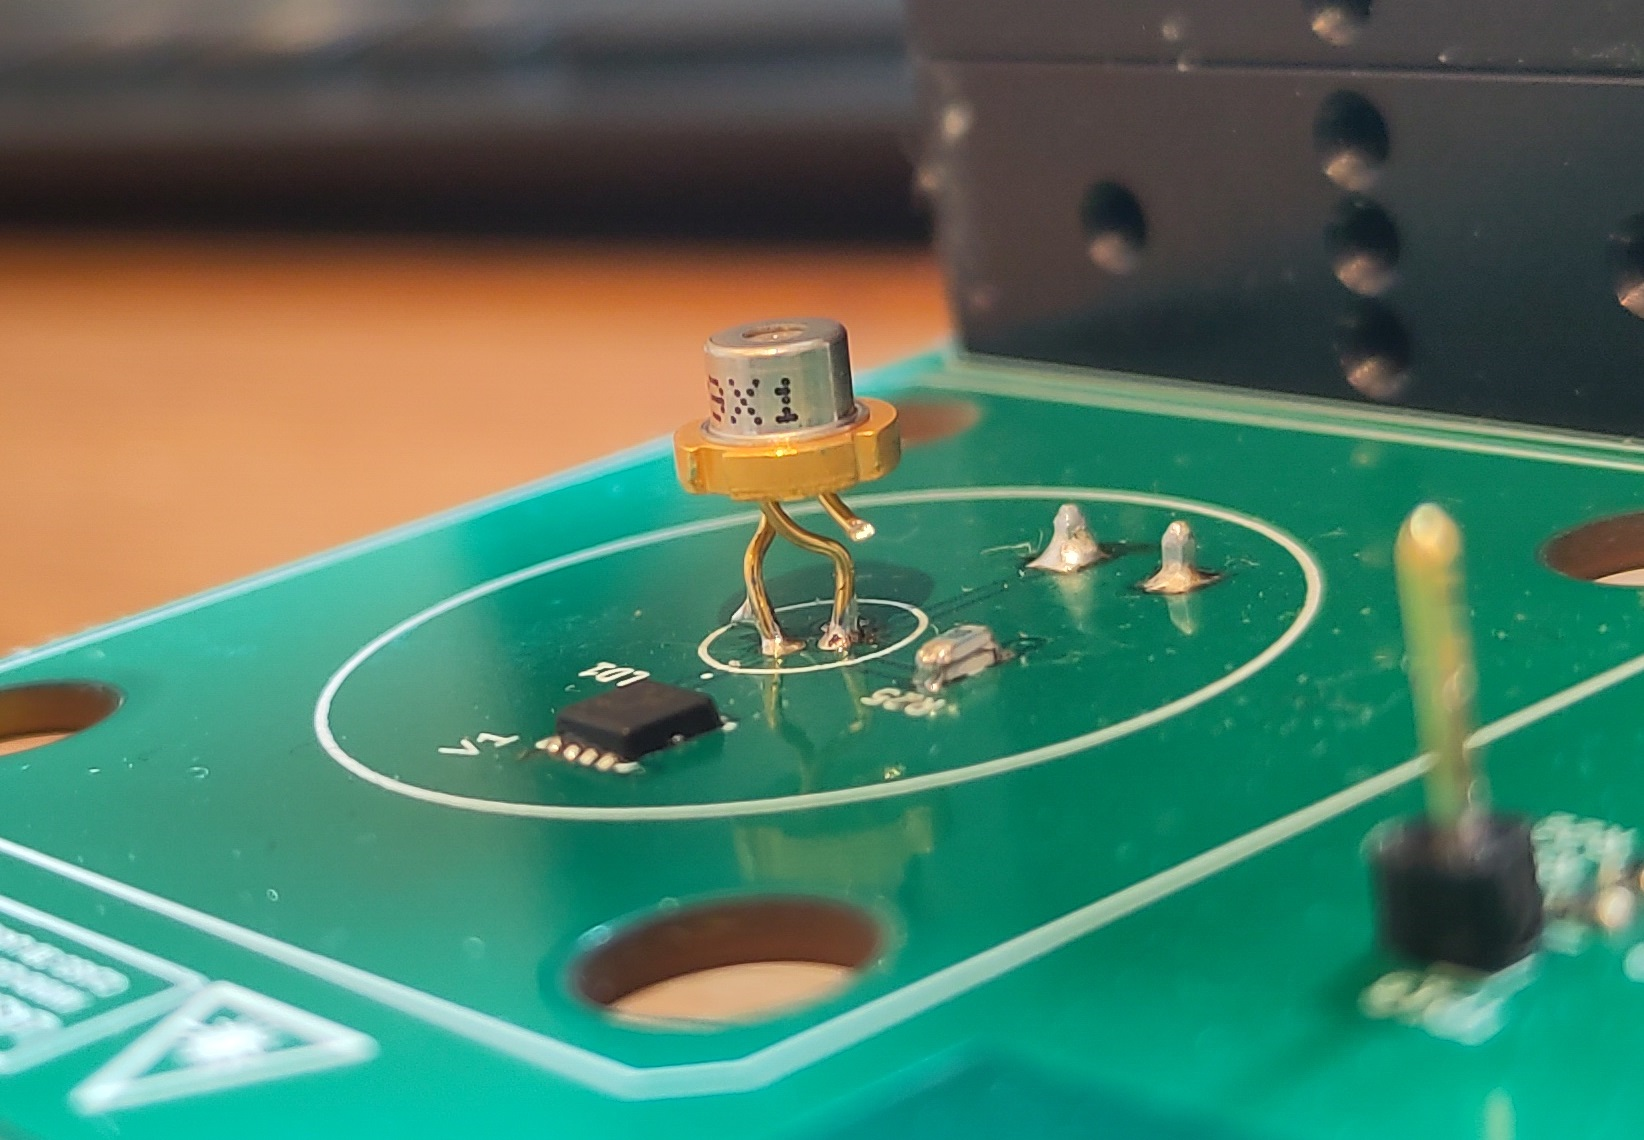
\includegraphics[width=0.6\textwidth]{graphics/laser_ausrichtung_angepasst.jpg}
    \caption{Laser-Ausrichtung angepasst}\label{fig:laser_ausrichtung_angepasst}
\end{figure}

Das \acrshort{dso}-Diagramm einer initialen Spiegel-Messung mit ca. 20~cm Distanz zum Spiegel ist in
Abbildung~\ref{fig:spiegel_initial} dargestellt. Es zeigt den Ausgang des Transimpedanzverstärkers. Zusätzlich, um die
Verzögerungszeit zu sehen, wurden auch die \acrshort{mcu}-Signale \lstinline|start_op| und \lstinline|LD_pulse| sowie
das Spannungspotential am Gate des FET aufgezeichnet.

\begin{figure}[H]
    \centering
    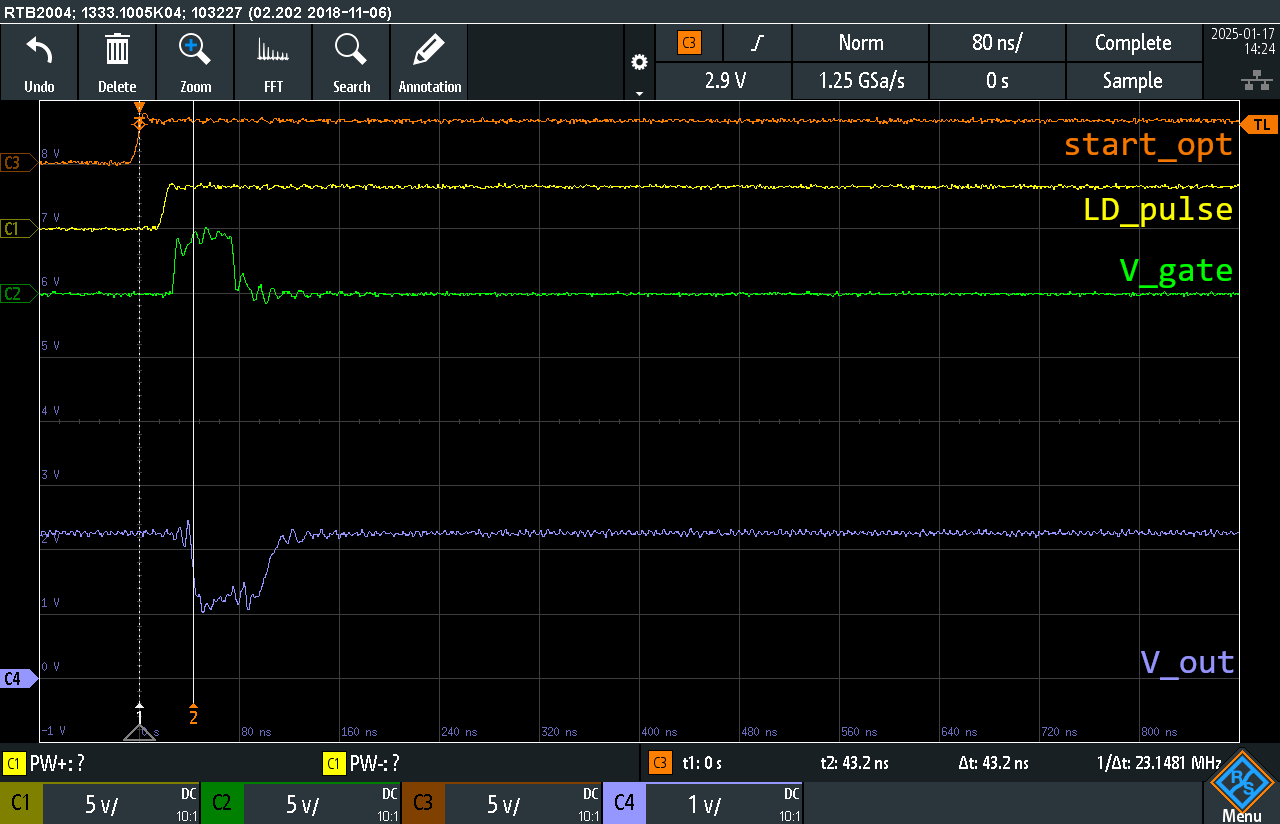
\includegraphics[width=\textwidth]{graphics/spiegel_initial.png}
    \caption{Initiale Spiegelmessung mit \acrshort{dso}}\label{fig:spiegel_initial}
\end{figure}

Mit dem Demonstrator wurden Messwerte für drei verschiedene Distanzen aufgezeichnet: 19~cm, 24~cm und 28.5~cm.

Die mit dem optischen \acrshort{tdc} erfassten Datenpunkte sind in
Abbildung~\ref{fig:spiegel_unterschiedliche_distanzen} dargestellt. Es wurden je ca. 300 Messwerte erfasst, die Liste
mit den Datenpunkten befindet sich im elektronischen Anhang.

\begin{figure}[H]
    \centering
    \includesvg[width=0.9\textwidth]{graphics/spiegel_unterschiedliche_distanzen.svg}
    \caption{Unterschiedliche Distanzen zum Spiegel - Plot}\label{fig:spiegel_unterschiedliche_distanzen}
\end{figure}

Die arithmetischen Mittelwerte und die Standardabweichungen sind in Tabelle~\ref{tab:spiegel_unterschiedliche_distanzen}
aufgelistet.

\begin{table}[H]
    \mytable
        {|l|l|l|}
        {\textbf{Distanz zum Spiegel} & \textbf{Mittelwert} & \textbf{Standardabweichung}}
        {\distance & \mean & \stddev}
        {tables/spiegel_unterschiedliche_distanzen.csv}
    \caption{Unterschiedliche Distanzen zum Spiegel - Statistische Grössen}\label{tab:spiegel_unterschiedliche_distanzen}
\end{table}

Es fällt auf, dass die Standardabweichungen relativ gross sind, dies hat insbesondere mit den beiden Clustern zu tun,
welche in Abbildung~\ref{fig:spiegel_unterschiedliche_distanzen} zu sehen sind. Die Ursache dieser Cluster ist unklar.
Eine Hypothese ist, dass diese mit dem \acrshort{dso} zusammenhängen. Es wurde festgestellt, dass das Anschliessen des
\acrshort{dso} einen signifikaten Einfluss auf den Offset der \acrshort{tdc}-Laufzeitwerte hat (ca. 10~ns). Eventuell
hat das \acrshort{dso} durch Sample und Hold einen zeitlich-abhängigen Einfluss auf die Messresultate -- je nach dem ob
der Lichtpuls gerade in einer Sample- oder Hold-Phase auf die Photodiode trifft. Die Ursache dieser Cluster sollten in
einer allfälligen weiterführenden Arbeit genauer analysiert werden.

Eine Spiegeldistanz-Änderung von 5~cm entspricht einer Längen-Änderung von 10~cm.

Die Messungen zeigen für diese Längen-Änderung von 10~cm eine Änderung der Laufzeit von durchschnittlich ca. 0.6~ns.

In Formel~\ref{eq:spiegel_unterschiedliche_distanzen} wird der theoretisch zu erwartende Laufzeit-Unterschied berechnet.

\begin{equation}\label{eq:spiegel_unterschiedliche_distanzen}
    \Delta ToF = \frac{\Delta L}{c} = \frac{10~cm}{3 \cdot 10^8~m/s} = 0.33~ns
\end{equation}
\myequations{Theoretisch erwartete Laufzeit-Änderung}

Dieser Unterschied (ca. Faktor 2) könnte mehrere Gründe haben:

1.) Eine mögliche Erklärung ist, dass die Flanke bei grösserer Distanz weniger steil wird und dadurch fälschlicherweise
eine etwas längere Laufzeit gemessen wird.

2.) Etwas anderes, das in Abbildung~\ref{fig:spiegel_unterschiedliche_distanzen} auffällt, ist ein Time-Drift während
dem Aufzeichnen der Messdaten bei 24~cm und 29~cm. Abbildung \ref{fig:spiegel_unterschiedliche_distanzen_linear} soll
dies verdeutlichen.

\begin{figure}[H]
    \centering
    \includesvg[width=0.9\textwidth]{graphics/spiegel_unterschiedliche_distanzen_linear.svg}
    \caption{Unterschiedliche Distanzen zum Spiegel - Plot mit linearer Interpolation}\label{fig:spiegel_unterschiedliche_distanzen_linear}
\end{figure}

Dieser Time-Drift kann aber den gemessenen Unterschied nicht schlüssig erklären.

Bemerkung: Der Spiegel musste sehr genau ausgerichtet werden und dann sehr stabil gehalten werden, um Resultate mit
relativ kleiner Standardabweichung (ca. 1~ns) messen zu können.

Bei Distanzen von mehr als 30~cm wird das \acrshort{tdc}-Signal unbrauchbar.

Dies hat damit zutun, dass die Photodiode ab dann nur noch wenig Licht empfängt und entsprechend einen kleinen
Lichtstrom generiert. Dies führt zu einer kleineren Aussteuerung am Ausgang des Transimpedanzverstärkers. Somit wird die
Schaltschwelle des Komparators nicht mehr oder nur noch ganz knapp erreicht.

Abbildungen~\ref{fig:spiegel_12cm_dso_ok} und \ref{fig:spiegel_30cm_dso_nok} sollen dies verdeutlichen.

\begin{figure}[H]
    \centering
    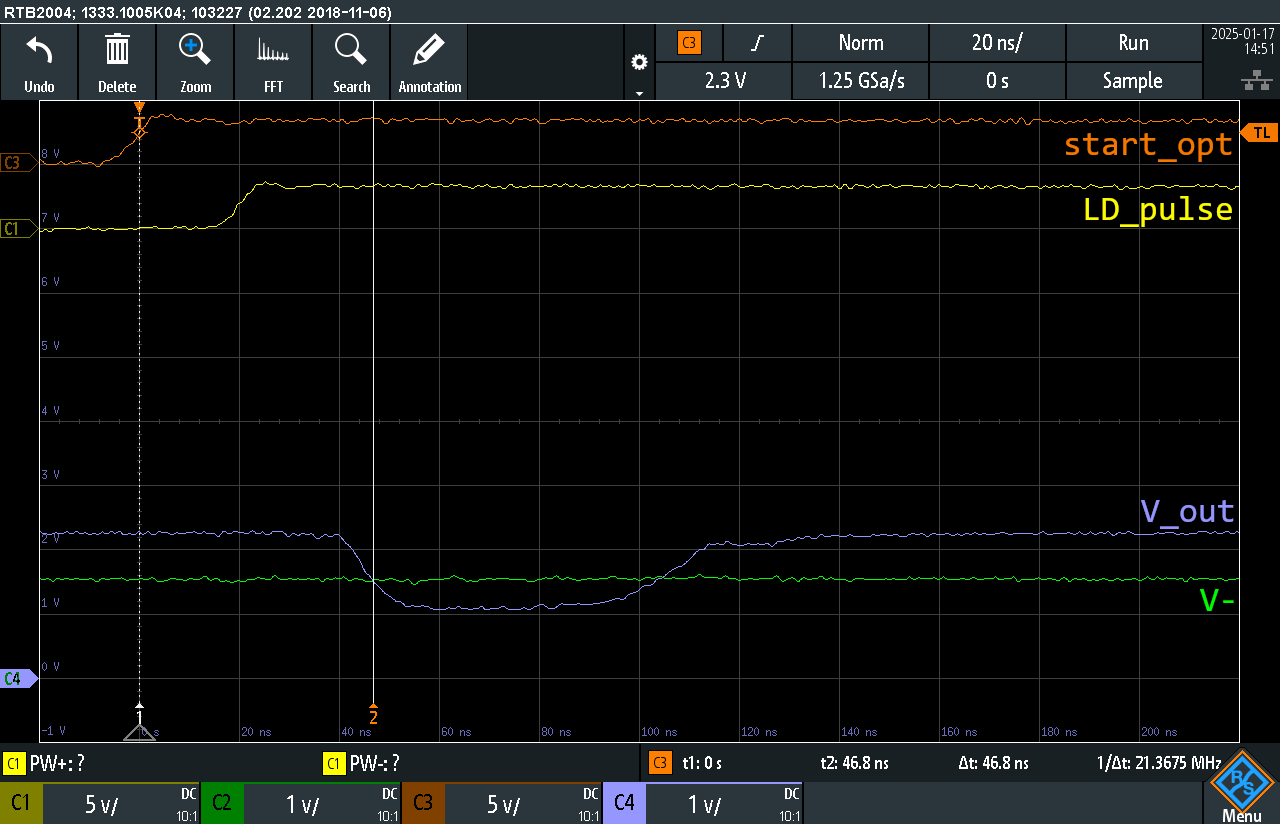
\includegraphics[width=\textwidth]{graphics/spiegel_12cm_dso_ok.png}
    \caption{\acrshort{tia}-Ausgang und Komparator-Schaltschwelle bei 12~cm}\label{fig:spiegel_12cm_dso_ok}
\end{figure}

\begin{figure}[H]
    \centering
    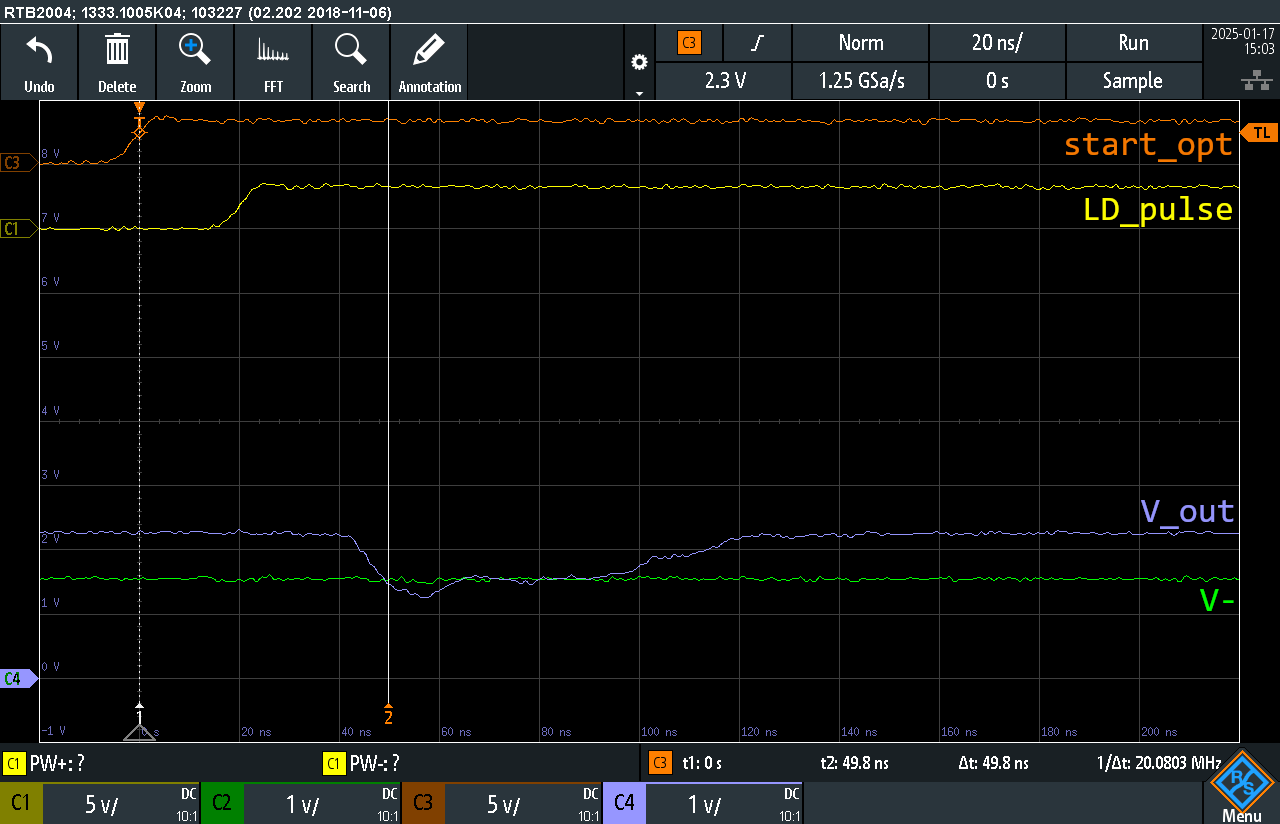
\includegraphics[width=\textwidth]{graphics/spiegel_30cm_dso_nok.png}
    \caption{\acrshort{tia}-Ausgang und Komparator-Schaltschwelle bei 30~cm}\label{fig:spiegel_30cm_dso_nok}
\end{figure}

Die Abbildungen zeigen, neben den \acrshort{mcu}-Signale \lstinline|start_op| und \lstinline|LD_pulse|, den Ausgang
des Transimpedanzverstärkers und die Komparator-Schaltschwelle.

Mögliche Verbesserungen dazu sind im Kapitel~\ref{sec:ausblick} aufgeführt.

\subsubsection{ToF-Messungen via Wand}\label{sec:messungen_wand}

Anstelle des in Kapitel~\ref{sec:messungen_spiegel} verwendeten Spiegels, werden in diesem Kapitel Messresultate mit
einer weissen Wand als Target aufgezeichnet. Es wurden Distanzen von ca. 10 bis 30~cm ausprobiert.

Es konnten mit diesem Setup in der kurzen zur Verfügung stehenden Zeit keine brauchbaren Messresultate erfasst werden.

Mögliche Verbesserungen dazu sind im Kapitel~\ref{sec:ausblick} aufgeführt.
